% Execution Time Comparison
\chapter{Experimental evaluation}
\label{chapter:exp_eval}
\section{Methodology}
\subsection{Dataset}
The dataset which will be used for benchmarking the optimization methods described in the previous chapters is the Wikipedia article dataset from Wikimedia available on hugging face\footnote{\url{https://huggingface.co/datasets/wikimedia/wikipedia}}.
This set contains over 6 million English articles from Wikipedia.
Instead of encoding all articles, which would result in almost 23 GB in vector embeddings, 1.2 million randomly selected articles were encoded resulting in 4.6 GB of embeddings for 1024 dimensions.
The data was converted by two different embedding models: The first one is the \texttt{\seqsplit{mixedbread-ai/mxbai-embed-large-v1}} model which is a very good performing model on the \textit{Massive Text Embedding Benchmark} (available here\footnote{\url{https://huggingface.co/spaces/mteb/leaderboard}}) paper.~\cite{muennighoff2023mtebmassivetextembedding} This is a vector angle optimized model \cite{li2024angleoptimizedtextembeddings} which should give binary quantization an advantage compared to traditional models. Additionally, this model embeds to 1024 vector dimensions and has 335M parameters. To have a comparison the dataset of 1.2 million articles will be encoded with the \texttt{\seqsplit{sentence-transformers/all-mpnet-base-v2}} model available here\footnote{\url{https://huggingface.co/sentence-transformers/all-mpnet-base-v2}}. This model maps the encoded text to 768 dimensions and has 109M parameters. It scores a bit worse on the \textit{Massive Text Embedding Benchmark} but is still a solid model (rank 117 of 476 for the sentence-transformer model compared to 35 of 476 for the mixedbread-ai model as of 2024-11-29).

Unless mentioned or annotated otherwise the results and figures presented in this chapter use the \texttt{\seqsplit{mixedbread-ai/mxbai-embed-large-v1}} model with retrieval for top 100 (k=100) documents.

To benchmark the different search methods a list containing 303 queries will be used. It contains long and short-, specific and unspecific-, pointless queries, etc.

\begin{table}[h]
    \centering
    \begin{tabular}{lcr}
        \toprule
        Method Name                                                          & Short Name             & Section                     \\
        \midrule
        naive float                                                          & float                  & \autoref{naivefloat}        \\
        Optimized Bianry with AVX2                                           & binary                 & \autoref{sec:optbinaryavx2} \\
        Optimized Int8 with AVX2                                             & int8                   & \autoref{sec:optint8avx2}   \\
        Float16                                                              & float16                & \autoref{sec:float16}       \\
        Mapped Float                                                         & mf                     & \autoref{sec:mappedfloat}   \\
        PCAX (X indicates reduction factor)                                  & pcaX                   & \autoref{sec:dimreduct}     \\
        \footnotesize Two-Step Binary + Float (X indicates rescoring factor) & twostep\_rfX | ts\_rfX & \autoref{sec:twostep}       \\
        \footnotesize Two-Step Binary + Mapped Float (X ind. resc. factor)   & ts\_mf\_rfX            & \autoref{sec:twostep}       \\
        \bottomrule
    \end{tabular}
    \caption{Short names used in plots}
    \label{shortnames}
\end{table}

\subsection{Evaluation metrics}
To evaluate the benchmark results the Jaccard index and NDCG will be used to compare the performance to the naive float implementation as a baseline. Additionally, the time taken for each search will be measured. This includes initialization of the results array, calculating the similarity for every embedding, sorting for top k results and returning the result. At last the theoretical memory usage will be calculated, see \autoref{memorycalc}.

\begin{table}[h]
    \centering
    \begin{tabular}{lcr}
        \toprule
        Method    & Formula for embedding size in bytes                                       \\
        \midrule
        general   & $sizeof(datatype) * vector\_dim * num\_embeddings$                        \\
        rescoring & $general(binary) + general(rescoring\_method) $                           \\
        PCA       & $general(datatype) + vector\_dim * (reduced\_dim + 1) * sizeof(datatype)$ \\
        \bottomrule
    \end{tabular}
    \caption{Calculation of memory used for different methods}
    \label{memorycalc}
\end{table}

\begin{table}[h]
    \centering
    \begin{tabular}{lccr}
        \toprule
        Method                         & Memory usage                                  & Mem. usage test Dataset \\
        \midrule
        float (including avx2 version) & $base$                                        & 4.58 GB                 \\
        binary                         & $\frac{base}{32}$                             & 0.14 GB                 \\
        int8                           & $\frac{base}{4}$                              & 1.14 GB                 \\
        float16                        & $\frac{base}{2}$                              & 2.29 GB                 \\
        mapped float                   & $\frac{base}{4} + 1kB$ for mapping table      & 1.14 GB                 \\
        PCA by factor $x$ (float)      & $\frac{base}{x} + d * (\frac{d}{x} + 1) * 4B$ & $\sim\frac{4.58 GB}{x}$ \\
        two-step binary+float          & $base + \frac{base}{32}$                      & 4.72 GB                 \\
        two-step binary+mapped float   & $base + \frac{base}{4} + 1kB$                 & 1.29 GB                 \\
        \bottomrule
    \end{tabular}
    \caption{Memory usage as ratio to baseline\\\footnotesize{d=vector dimension}}
\end{table}

\subsection{Testing environment}
All benchmarks were recorded on Linux using kernel version 6.11. Specifically version \texttt{\seqsplit{6.11.10-300.fc41.x86\_64}} shipped by fedora.
The test system has an AMD 5950X CPU (16C/32T) with disabled turbo boost to get a consistent frequency of 3.4GHz.
Furthermore, 128 GB of dual-channel/quad-rank DDR4 SDRAM running at 3600MTs/1800MHz with CL18 was used.

\section{Expected Outcome}
No implementation can have the same accuracy as the float32 variants as every type of quantization and dimension has some kind of information loss.
The binary method should be by far the fastest as it has very little data to work through, resulting from its heavy quantization, and efficient multiplication method. In return the accuracy should be fairly low. The float16 should be fairly good as using it for machine learning is already quiet common.
The int8 implementation should be around 2 to 4 times faster than the optimized float32 version, as it does 16 multiplications at once compared to 8 and integer math can be faster depending on architecture. The mapped float implementation should have good accuracy, better than int8 but worse than float16 as its accuracy is much higher. The performance can be good if it's not bottlenecked by the random access latency on the mapping table.
The search speed on the PCA variants should scale linear as the dimension decreases. PCA2 should decrease the search speed to about half (plus a little overhead) compared to the AVX2 float variant, as they both use the same implementation. With the only difference that PCA has the applied dimension reduction. The accuracy for the PCA searchers is hard to predict, but if there are redundant dimensions they should perform quiet good.

\section{Results and Analysis}
\subsection{Search Time comparison}
\begin{figure}[h]
    \makebox[\textwidth][c]{%
        \begin{minipage}{0.49\widefigwidth}
            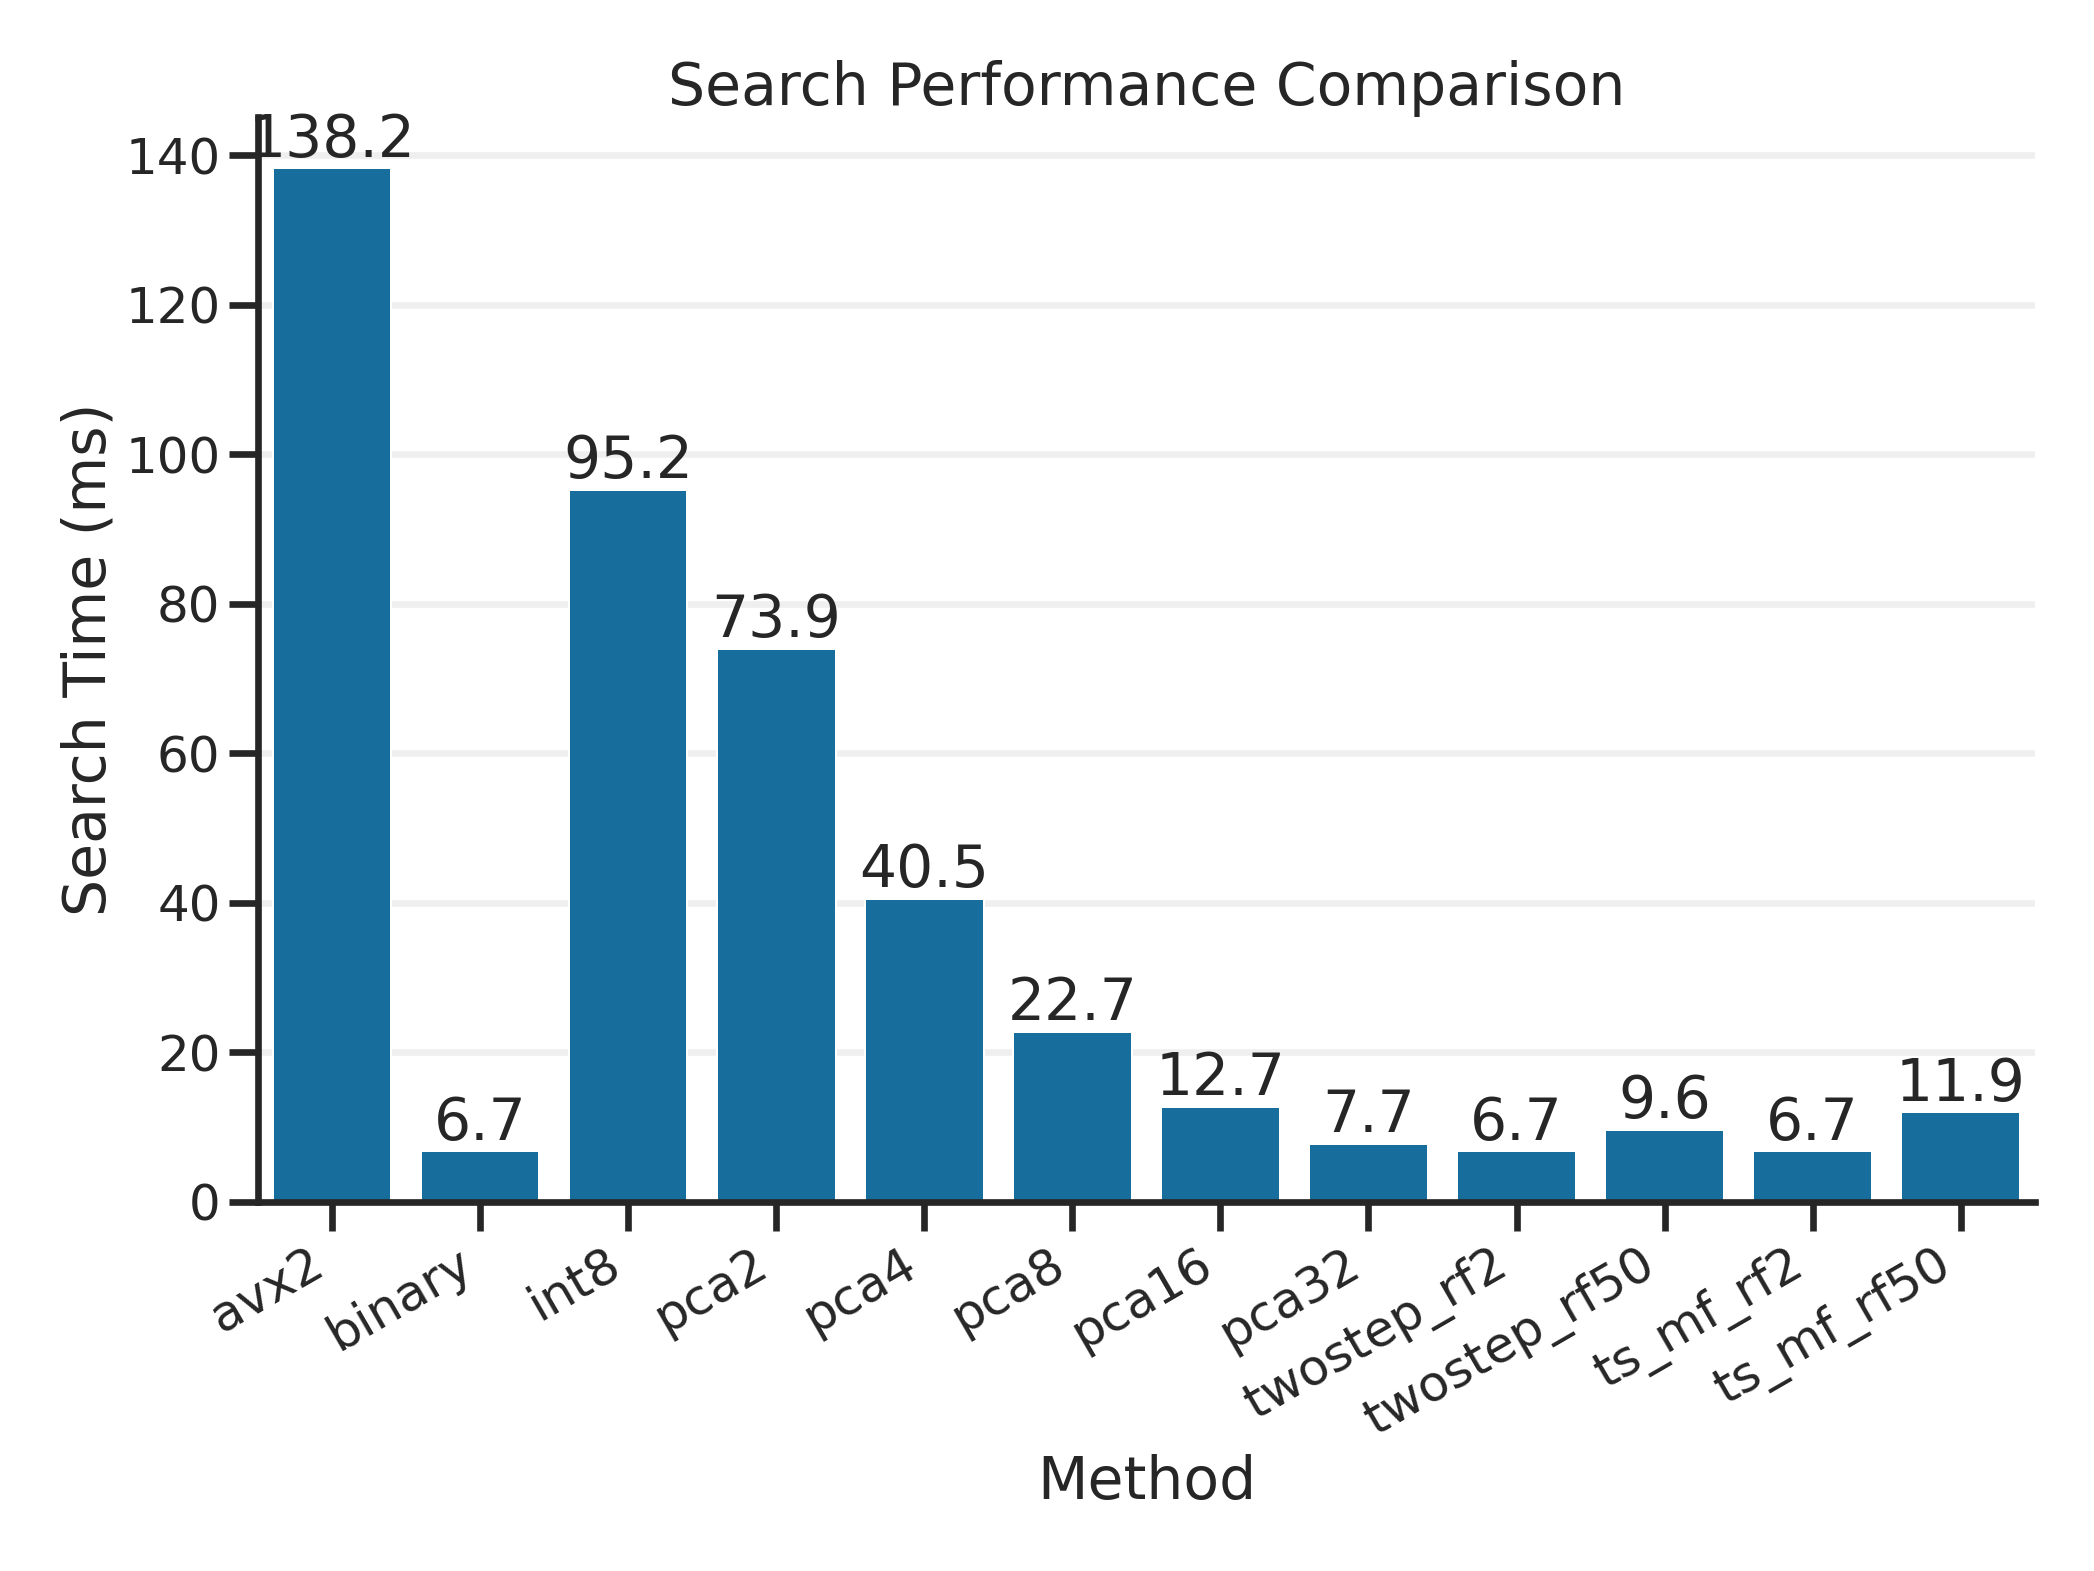
\includegraphics[width=0.49\widefigwidth]{bilder/plots/performance_comparison_dim1024_k100_q.png}
            \vspace{-1cm}
            \caption{Search Speed vec\_dim=1024}
            \label{searchspeed}
            \centering
            \small{float (1100 ms) and mapped float (540 ms) ommited}
        \end{minipage}
        %\hfill
        \begin{minipage}{0.49\widefigwidth}
            \vspace{-0.375cm}
            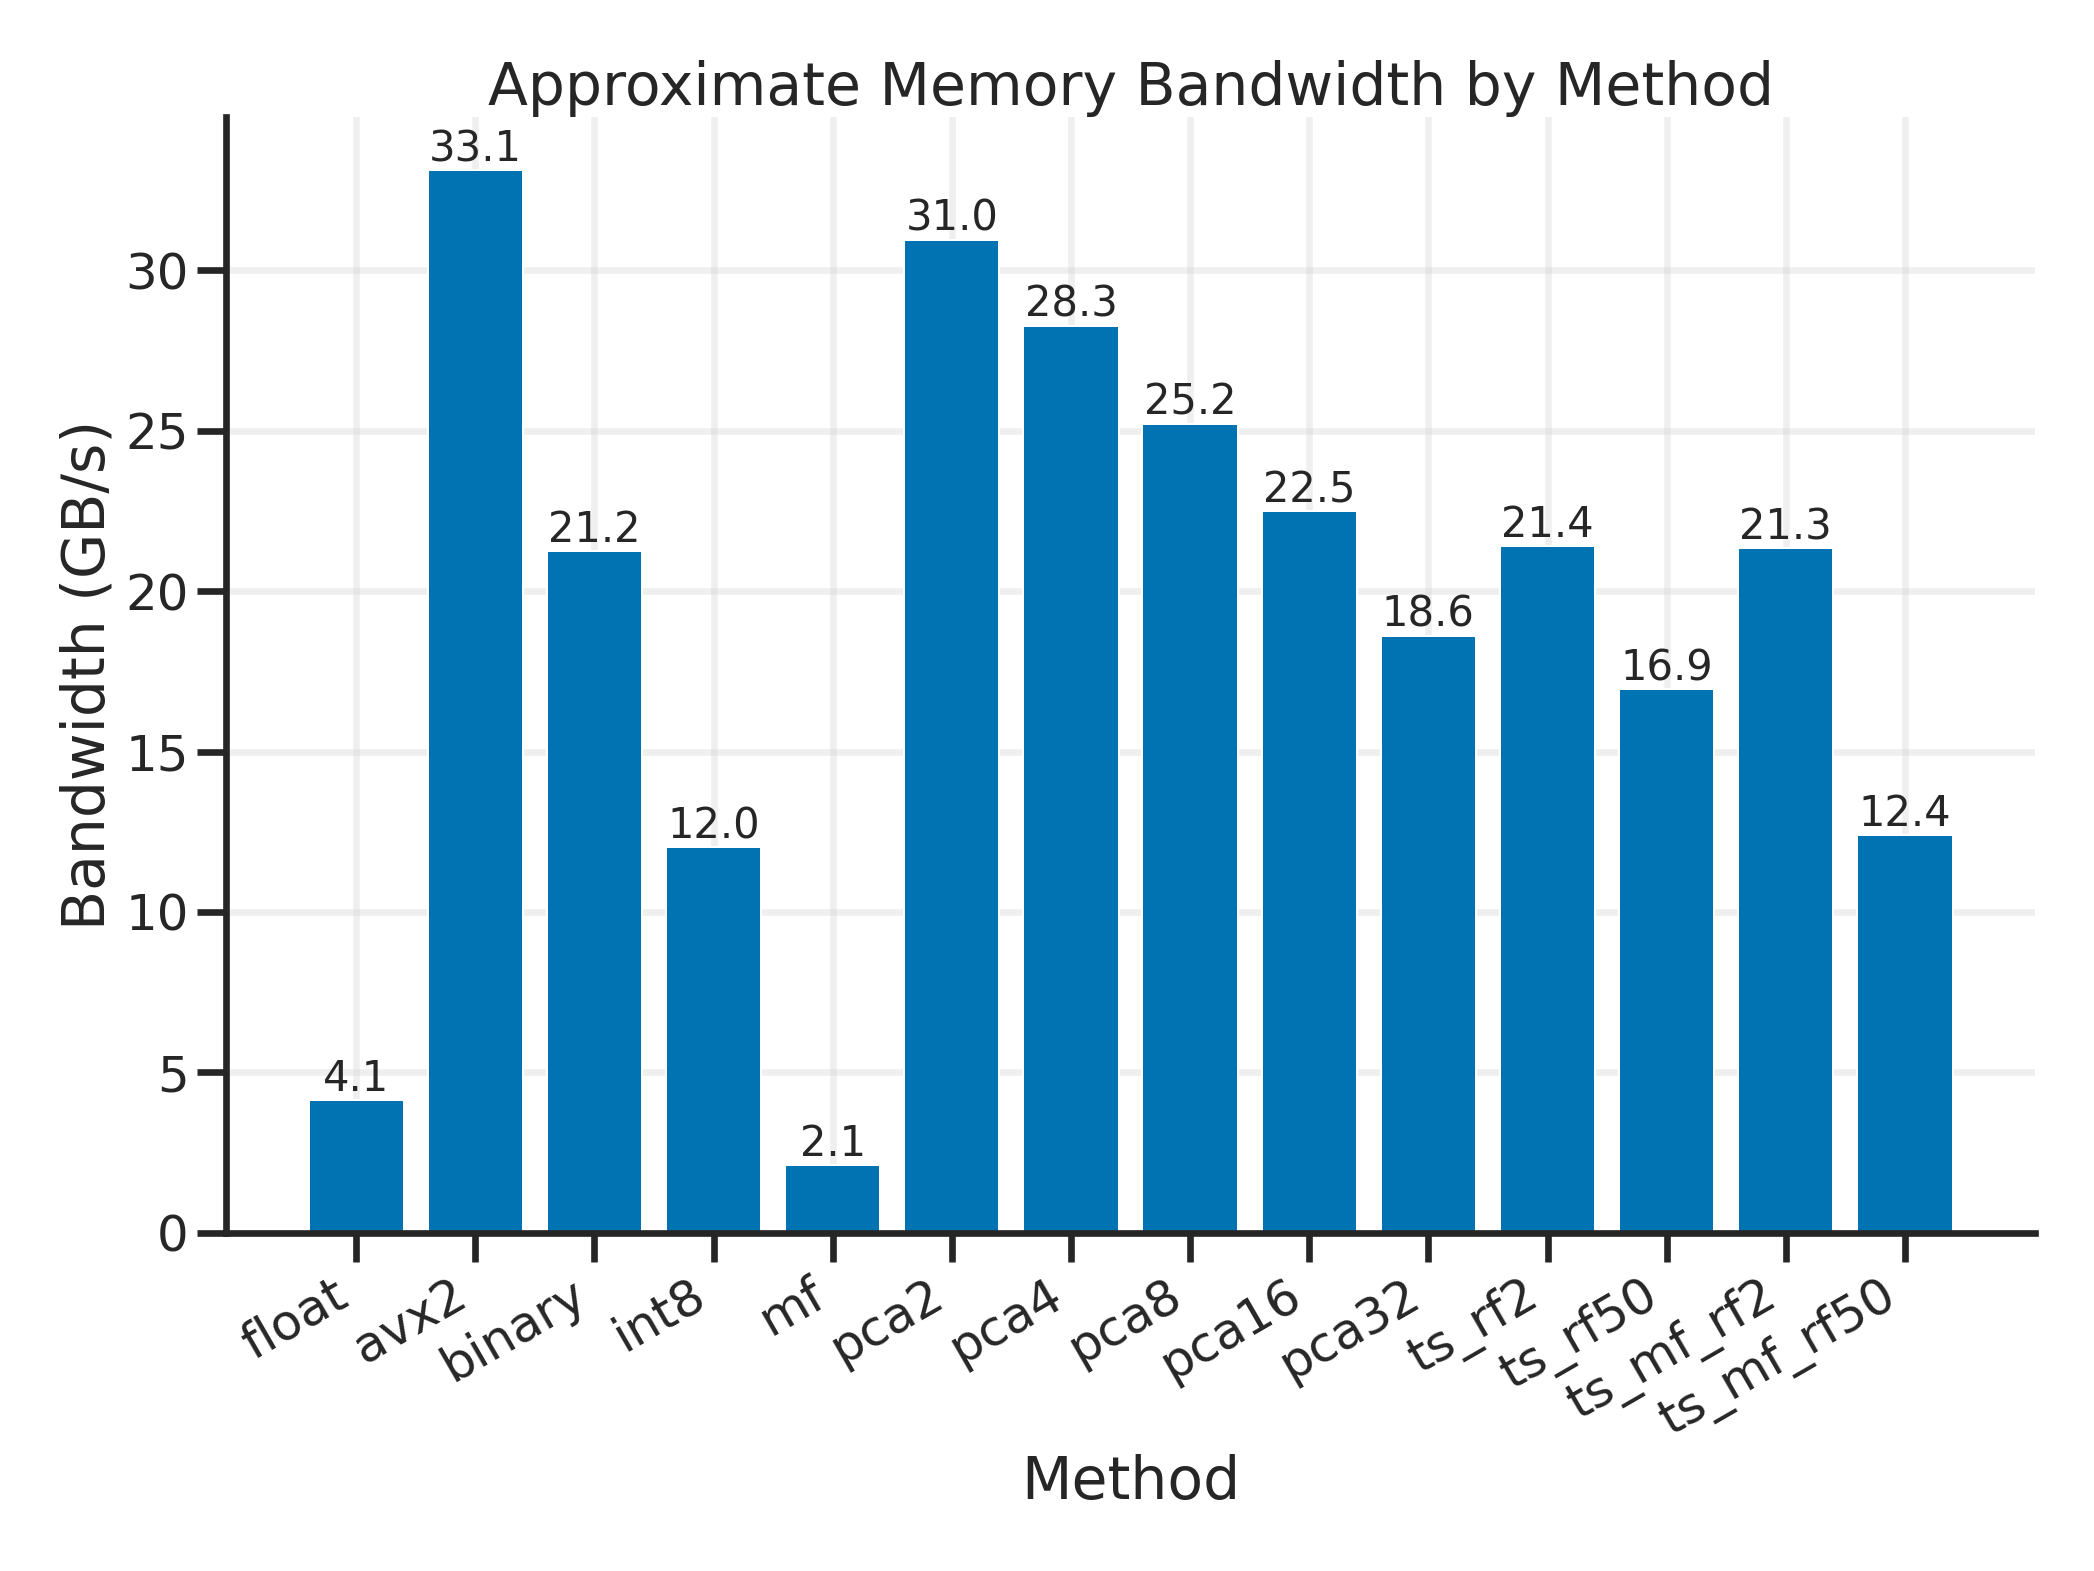
\includegraphics[width=0.49\widefigwidth]{bilder/plots/memory_bandwidth_benchmark_dim1024_k100_q.png}
            \vspace{-1cm}
            \caption{Memory bandwidth vec\_dim=1024}
            \label{memorybandwidth}
        \end{minipage}
    }
\end{figure}
Starting with \autoref{searchspeed}: As expected the AVX2 optimized version is much faster than the naive implementation. The fact it's 8 times faster, taking only 138.2 ms compared to 1100 ms for float, shows that this implementation makes efficient use of the AVX2 instructions.

The binary implementation, which also uses AVX2, is over 23 times faster than the AVX2 float equivalent and over 160 times faster than the baseline float implementation. Which makes sense, because it only has to iterate through $1/32$th of the data and uses efficient nor, xor and popcount instructions.

With 95 ms The int8 implementation is slower than expected. But that is likely due to the fact that AVX2 can't multiply 32 int8 values at once. It has to extract the lower/higher 128 bits, extend them to 16bit and then do 2 multiplications for the high and low values. After that it has to build the horizontal sum and add the high and low multiplication result to the running sum. This is a significant amount of instructions compared to the AVX2 float implementation where 32 floats are multiplied and added to the running sum by just 4 FMA instructions.

The PCA variants perform quiet well. The dimension reduction to half almost doubles the search speed compared to the float AVX2 implementation, which makes sense, given the fact that the vectors only have half the dimensions. The other PCA factors almost scale linearly as well. Which suggests, that the overhead from the functions involved calculating the similarities is very low. PCA4 is more than 2 times faster than int8 which has to go through the same amount of data. This shows that AVX2 doesn't really perform well at multiplying int8 values.

The two-step method based on the binary and float AVX2 implementation is very close to the pure binary search time. Even for high numbers of retrieved documents and rescoring factors, the amount of embeddings the second step method has to search is very small, e.g. 5000 for k=100 and rescoring factor of 50 (like in \autoref{searchspeed}), compared to the total number of embeddings.

With 540ms the mapped float searcher has the second-worst search time after the naive float. The reason for this being, that the CPU prefetcher can only predict the int8 values that will be loaded next. But after this gather instructions are used to load the corresponding float values from the mapping table. Even though it's very small (1 KB) and likely stays in L1 cache the entire time, even the very low L1 cache latency of around 1ns adds up: Taking the benchmarked dataset with 1.2M embeddings with 1024 dimensions it would take $10^{-9} s * 1024 * 1.2 * 10^{6} / 8 = 153.6 ms$ just to load the float values for the embeddings. And this makes the assumption, that loading 8 float values at once takes 1ns. In conclusion, this methods' reliance on random memory access slows the search significantly. This is also seen in the low memory bandwidth in \autoref{memorybandwidth}.

Finally, the two-step method using binary and the mapped float performs similar to binary just like the two-step method that uses full accuracy search in the second step. Only as the rescoring factor increases it takes slightly longer than its competitor. That happens, because the mapped float searcher is much slower than the avx2 searcher and as the rescoring factor increases the speed of the second-step searcher becomes more relevant. Nonetheless, this search method performs really well, as long the rescoring factors are reasonable.

\subsection{Accuracy Analysis}
The AVX2 implementation has perfect accuracy as seen in \autoref{accuracyheatmapone}. But one can spot one outlier for the Jaccard index and NDCG score in \autoref{boxjaccardsearchersone} and \autoref{boxndcgsearchersone} respectively. But that is likely due to the fact that the AVX2 implementation can actually be more accurate with the fused multiply add instruction, which eliminates one rounding step.

\begin{figure}[h]
    \makebox[\textwidth][c]{%
        \begin{minipage}{0.49\widefigwidth}
            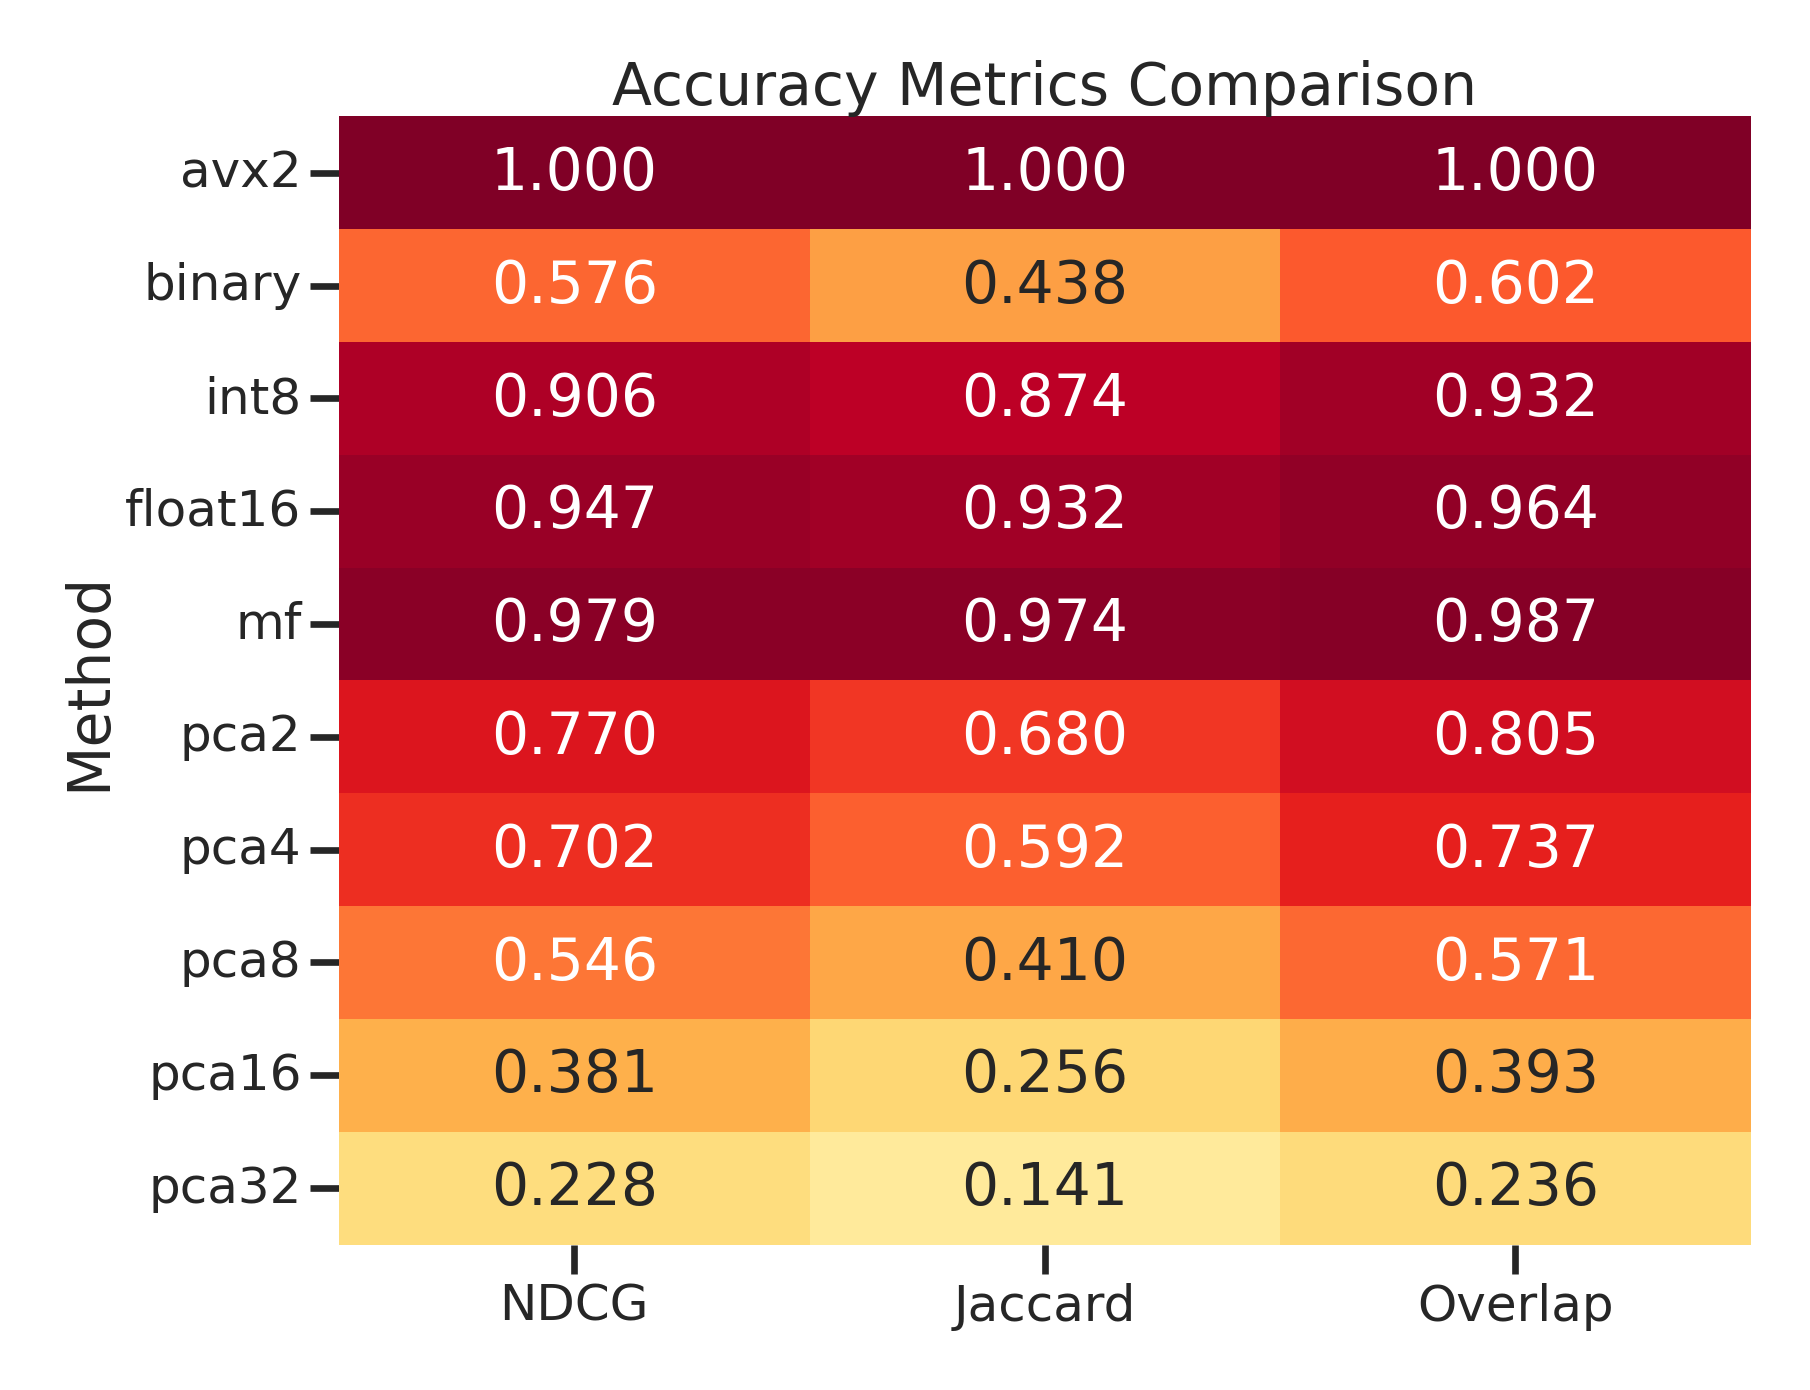
\includegraphics[scale=1]{bilder/plots/accuracy_heatmap_dim1024_k100_q.png}
            %\vspace*{-1cm}
            \caption{Accuracy of searchers}
            \label{accuracyheatmapone}
        \end{minipage}
        %\hfill
        \begin{minipage}{0.49\widefigwidth}
            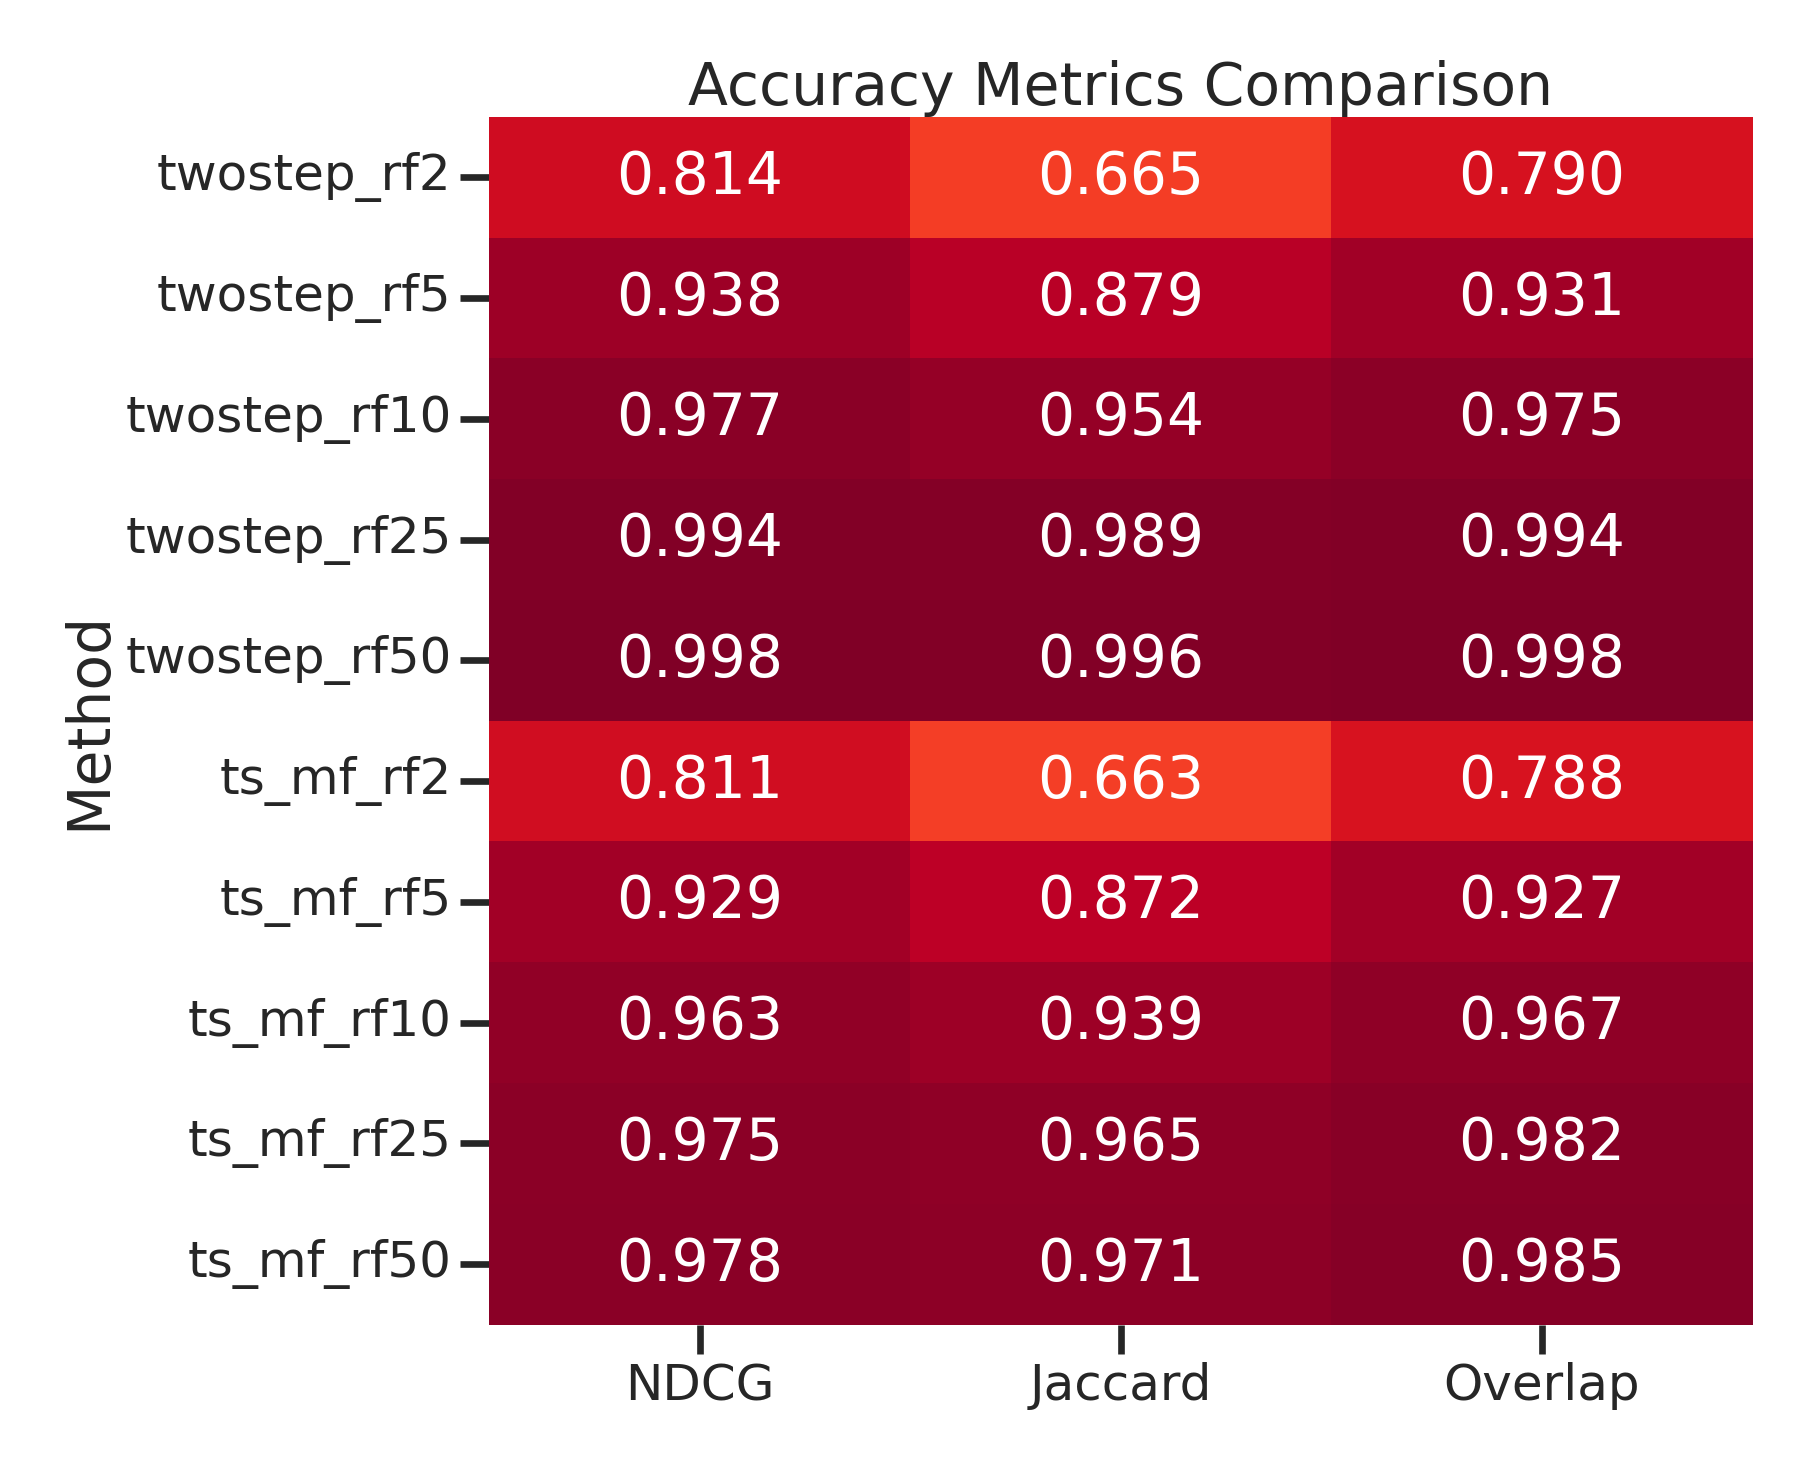
\includegraphics[scale=1]{bilder/plots/accuracy_heatmap_dim1024_k100_q_twostep.png}
            %\vspace*{-1cm}
            \caption{Accuracy of two-step searchers}
            \label{accuracyheatmaptwo}
        \end{minipage}
    }
\end{figure}

\begin{figure}[h]
    \makebox[\textwidth][c]{%
        \begin{minipage}{0.49\widefigwidth}
            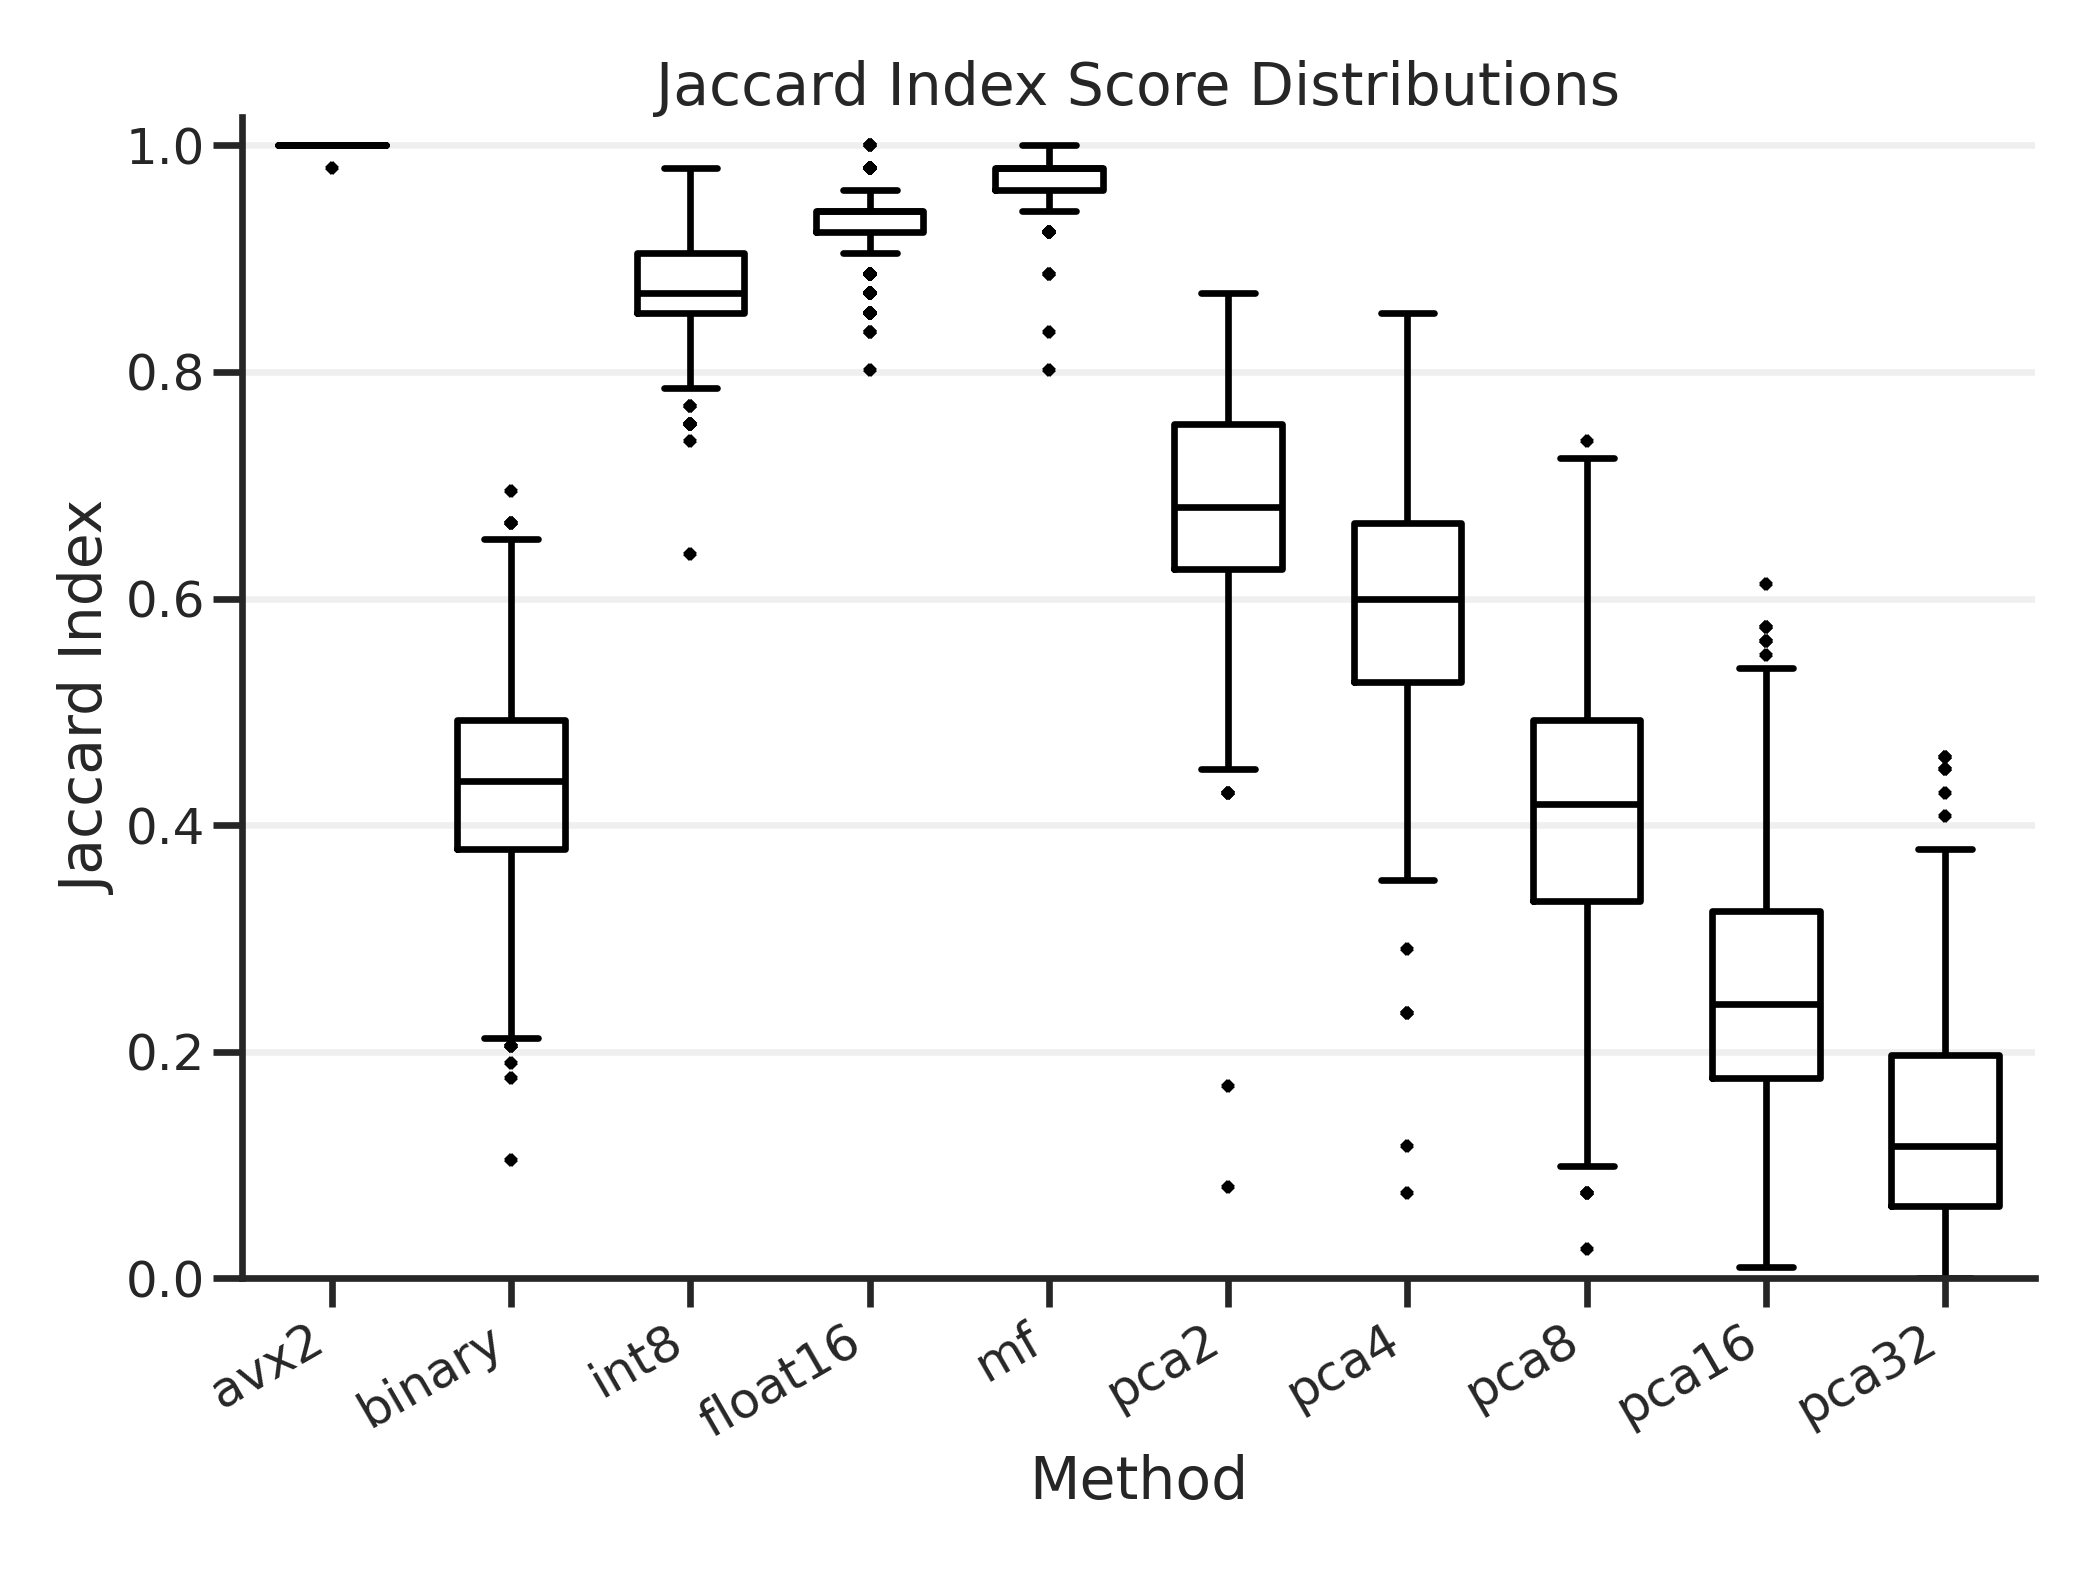
\includegraphics[width=0.49\widefigwidth]{bilder/plots/jaccard_boxplots_dim1024_k100_q.png}
            \vspace*{-1cm}
            \caption{Jaccard index of searchers}
            \label{boxjaccardsearchersone}
        \end{minipage}
        %\hfill
        \begin{minipage}{0.49\widefigwidth}
            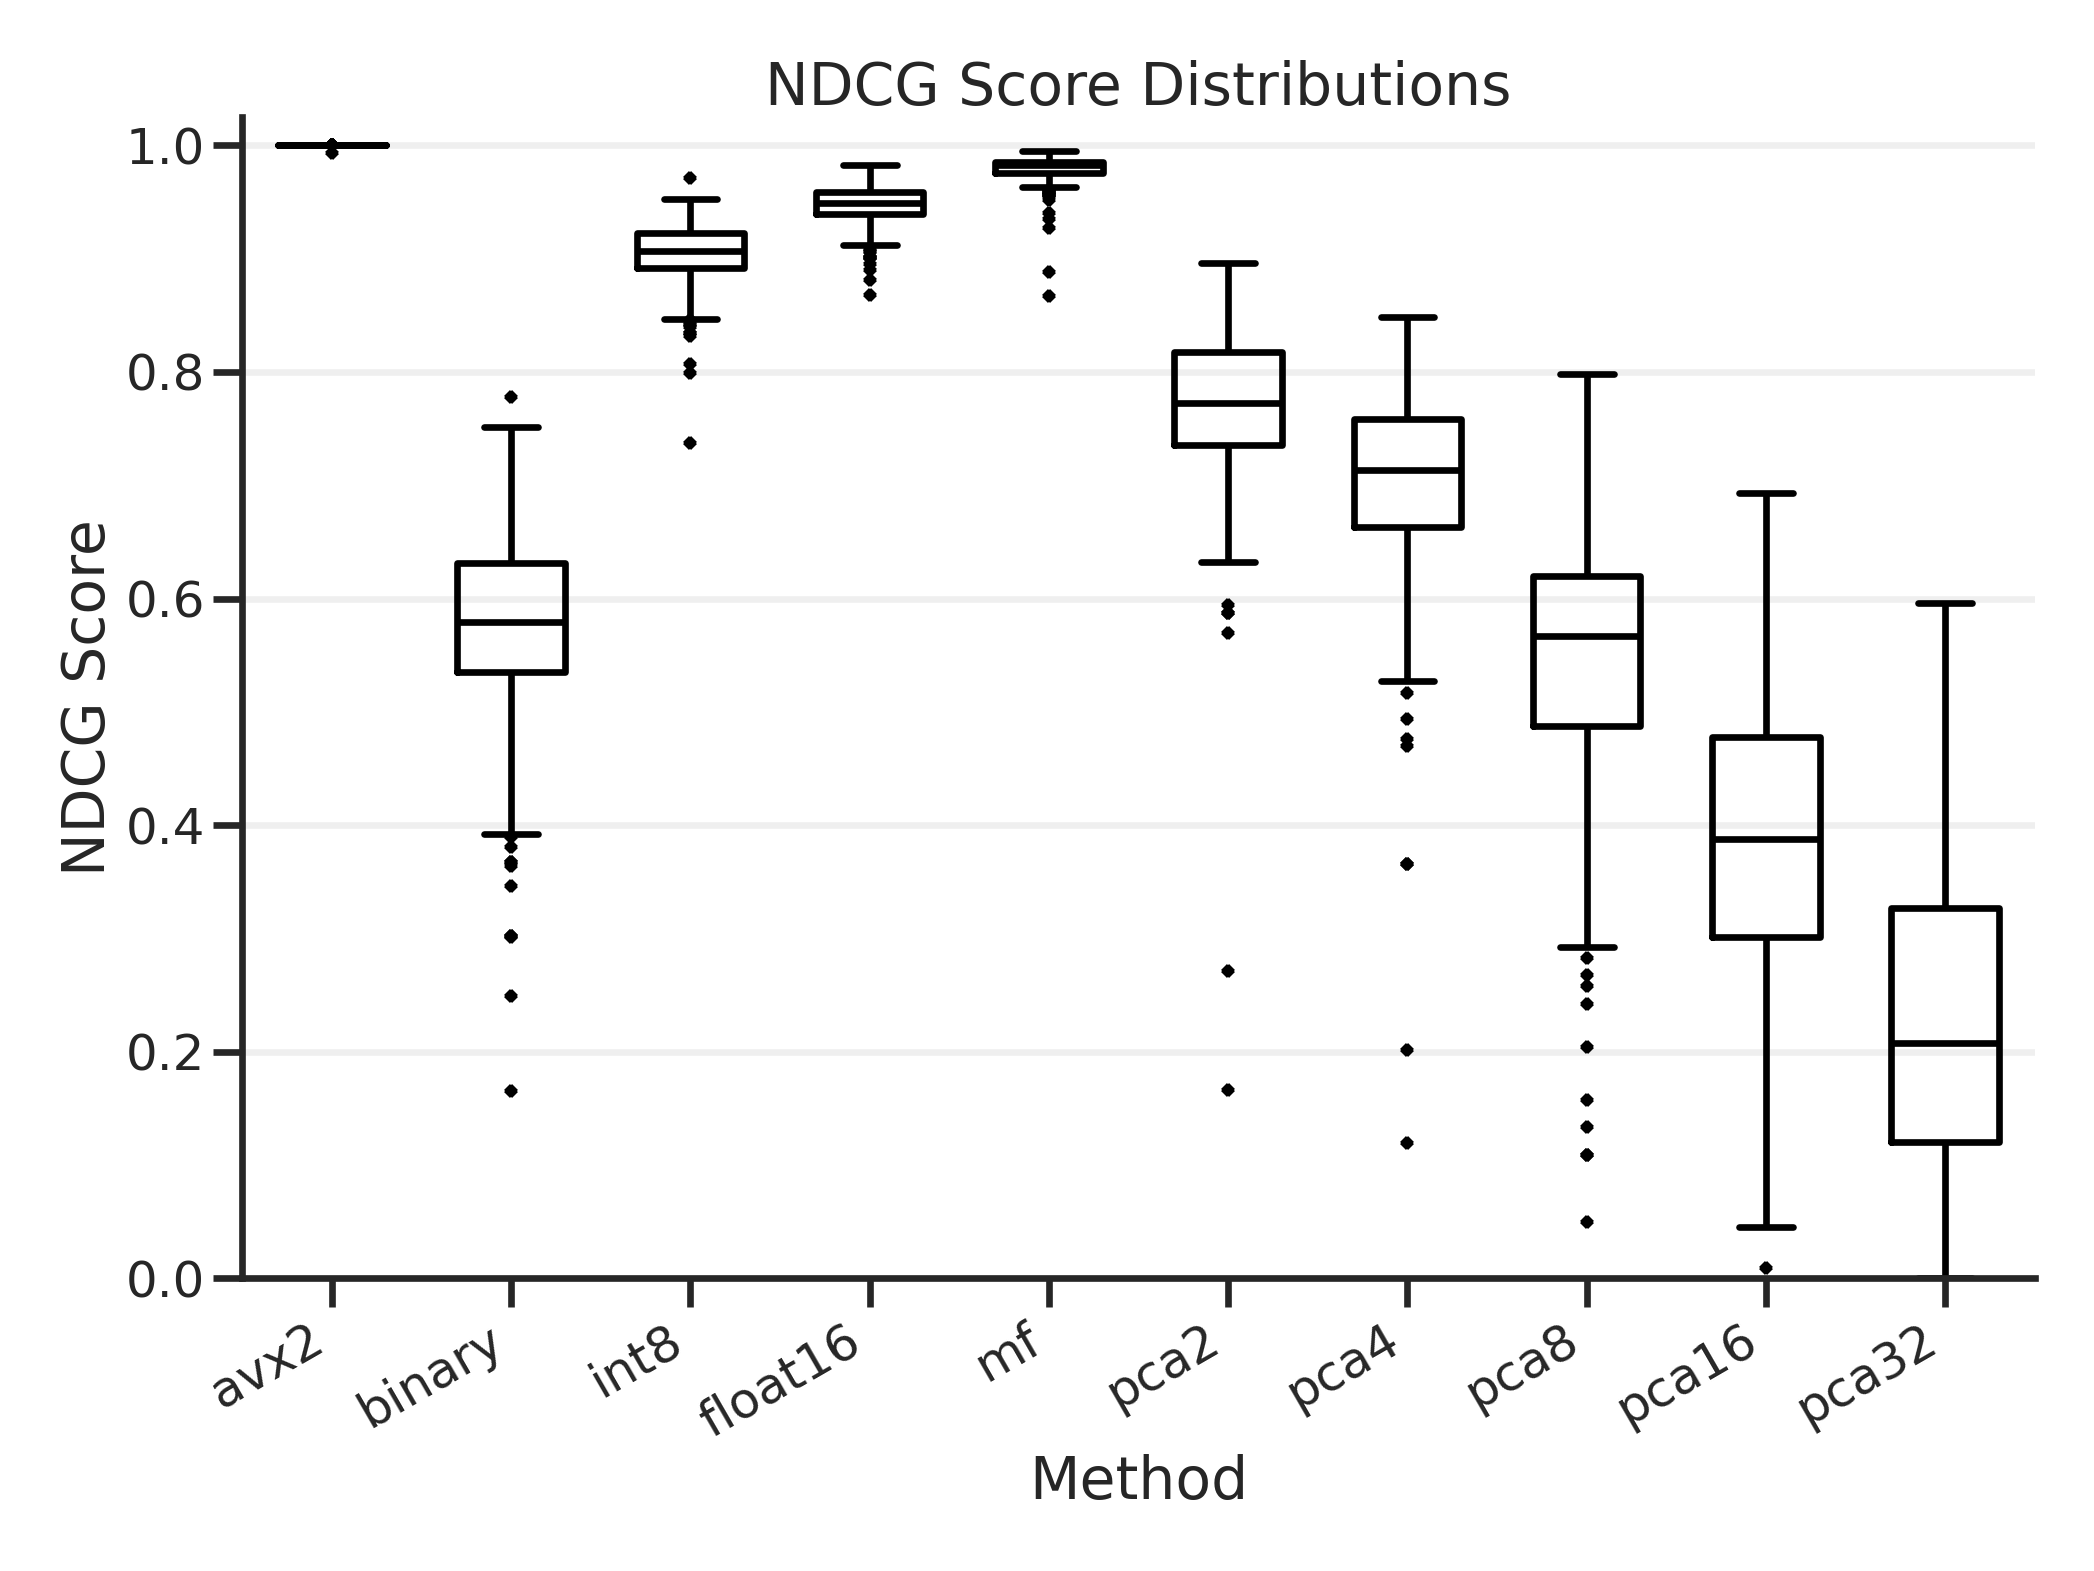
\includegraphics[width=0.49\widefigwidth]{bilder/plots/ndcg_boxplots_dim1024_k100_q.png}
            \vspace*{-1cm}
            \caption{NDCG score of searchers}
            \label{boxndcgsearchersone}
        \end{minipage}
    }
\end{figure}

The binary searcher performs decent with an average NDCG of 0.576 and Jaccard index of 0.438 when considering its heavy quantization, the fast search time and low memory usage. The PCA32 method, for example, uses the same amount of memory but has a much lower score which makes it useless in comparison to the binary searcher. The NDCG being higher than the Jaccard index indicates that the binary searcher also retrieves the important documents quiet reliably. In the box plots in \autoref{boxjaccardsearchersone} and \autoref{boxndcgsearchersone} show some outliers close to, and below 0.2 Jaccard index and slightly above 0.2 NDCG. This means that for some queries it can be unreliable on its own.


The int8 based searcher performs well with an average NDCG of 0.9 and Jaccard index of 0.87. It performs exclusively above the binary searcher. The outliers are also a lot less drastic. Especially the NDCG stays above 0.8 for all queries except one.

Float16 or half precision float has very good average accuracy scores \autoref{accuracyheatmapone}. The box plots in \autoref{boxjaccardsearchersone} and \autoref{boxndcgsearchersone} also show it performing very good. Especially the first and third quartile have a very close range and stay above 0.92 Jaccard index and 0.94 NDCG. The outliers are also still very good with at least 0.8 Jaccard index and 0.87 NDCG. This makes it suitable to fully replace the float32 approach as it gives good memory savings, reliable results and is much faster on supported hardware.

Even better performs the mapped float searcher. On average, it gets close to perfect scores (\autoref{accuracyheatmapone}). The outliers are no worse than the float16 outliers and the lower percentiles are above 0.96 for both metrics. This makes it the most accurate quantization tested.

The variants with PCA dimension reduction applied to the embeddings mostly perform worse than methods with the similar memory usage and search speed. Int8 is more accurate than PCA2 and only uses half the memory, while PCA2 only got a slight speed advantage. When comparing it to the binary search method, we see, that PCA8 performs worse while taking 3 times longer and using quadruple the memory. The bad performance when using PCA for embeddings is also mentioned here.~\cite{thakur2023injectingdomainadaptationlearningtohash}

\begin{figure}[h]
    \makebox[\textwidth][c]{%
        \begin{minipage}{0.49\widefigwidth}
            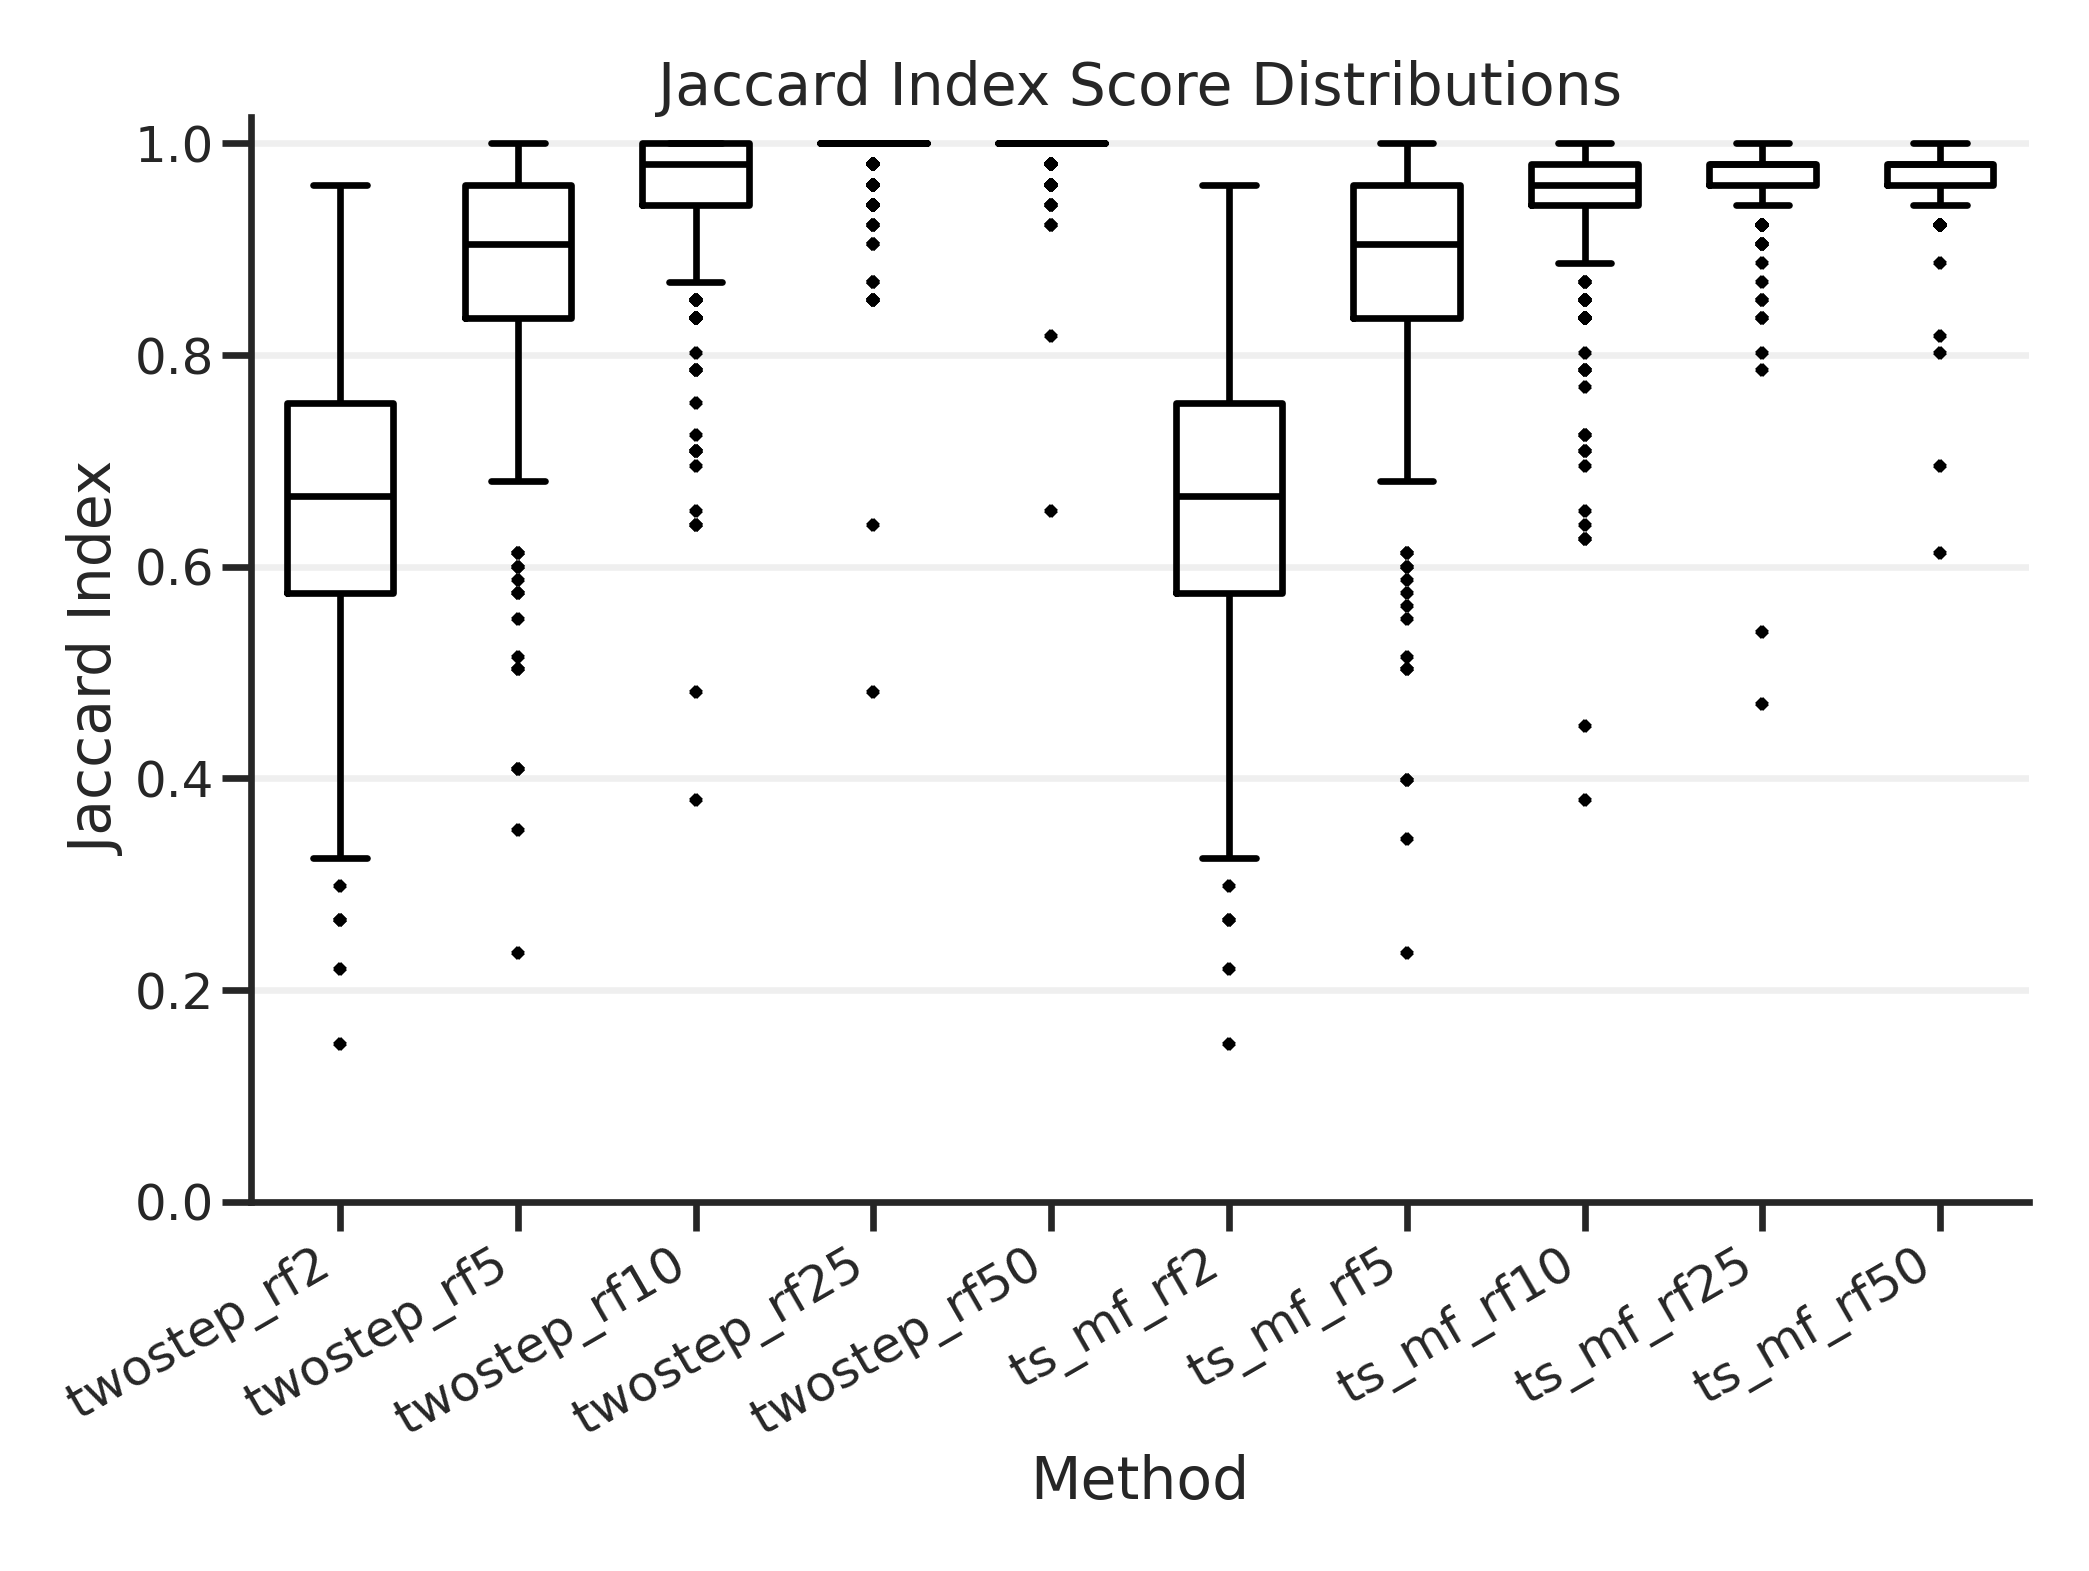
\includegraphics[width=0.49\widefigwidth]{bilder/plots/jaccard_boxplots_dim1024_k100_q_twostep.png}
            \vspace*{-1cm}
            \caption{Jaccard index of two-step searchers}
            \label{boxjaccardsearcherstwo}
        \end{minipage}
        %\hfill
        \begin{minipage}{0.49\widefigwidth}
            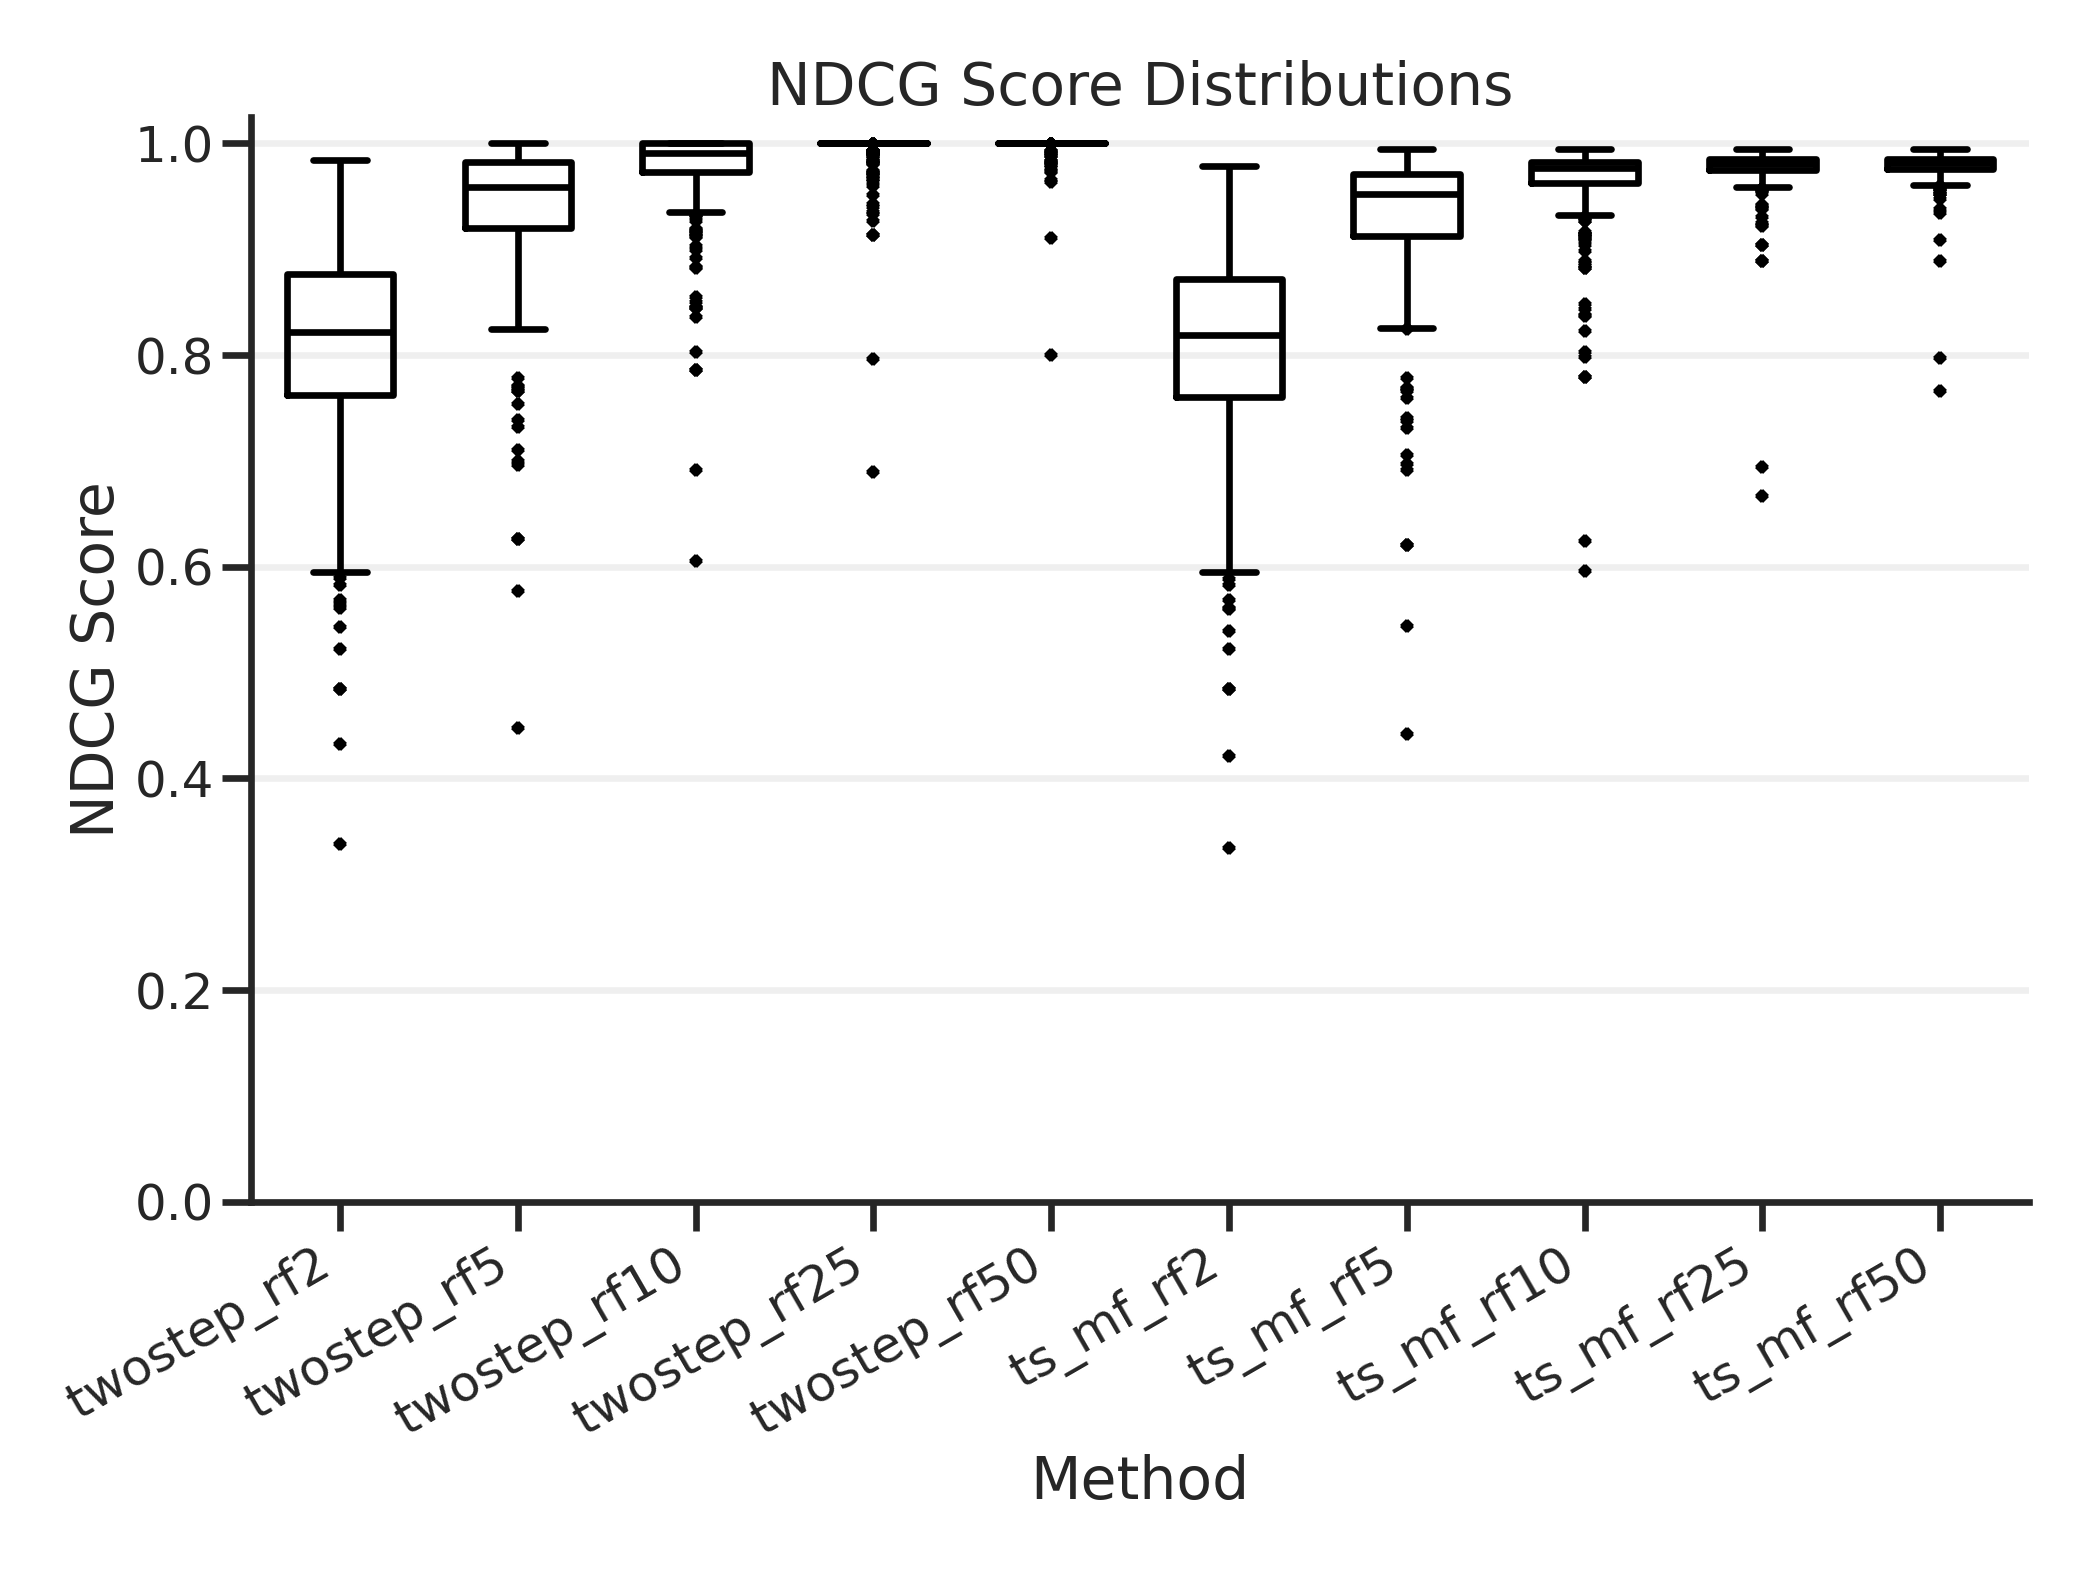
\includegraphics[width=0.49\widefigwidth]{bilder/plots/ndcg_boxplots_dim1024_k100_q_twostep.png}
            \vspace*{-1cm}
            \caption{NDCG score of two-step searchers}
            \label{boxndcgsearcherstwo}
        \end{minipage}
    }
\end{figure}

Both two-step methods (binary+float and binary+mapped float) perform really well. Especially with rescoring factors of 10 and higher. For a rescoring factor of 10 they have a first quartile NDCG score of 0.96 and 0.97 respectively. The outliers from the binary searcher still exists and only get slightly better as the rescoring factor increases.
With a rescoring factor of 25 or higher the binary+float searcher mostly gets perfect scores, except for the outliers. The score for the binary+mapped float searcher is capped by the mapped float searcher which is still very high.

\subsection{Accuracy vs Rescoring Factor}

As mentioned in the previous section the search time increases when increasing the rescoring factor. The increase in time is linear as seen in \autoref{time_ndcg_jaccard_vs_rescoring_factor_bf} and \autoref{time_ndcg_jaccard_vs_rescoring_factor_bmf}. The search time overall stays very low as even with high rescore factors the number of prefiltered embeddings is very small compared to the total number of embeddings. At a rescoring factor of 25 the score is very close to the full search equivalent of the second method. The only point in increasing it further is to reduce outliers.
\begin{figure}[h]
    \makebox[\textwidth][c]{%
        \begin{minipage}[t]{0.49\widefigwidth}
            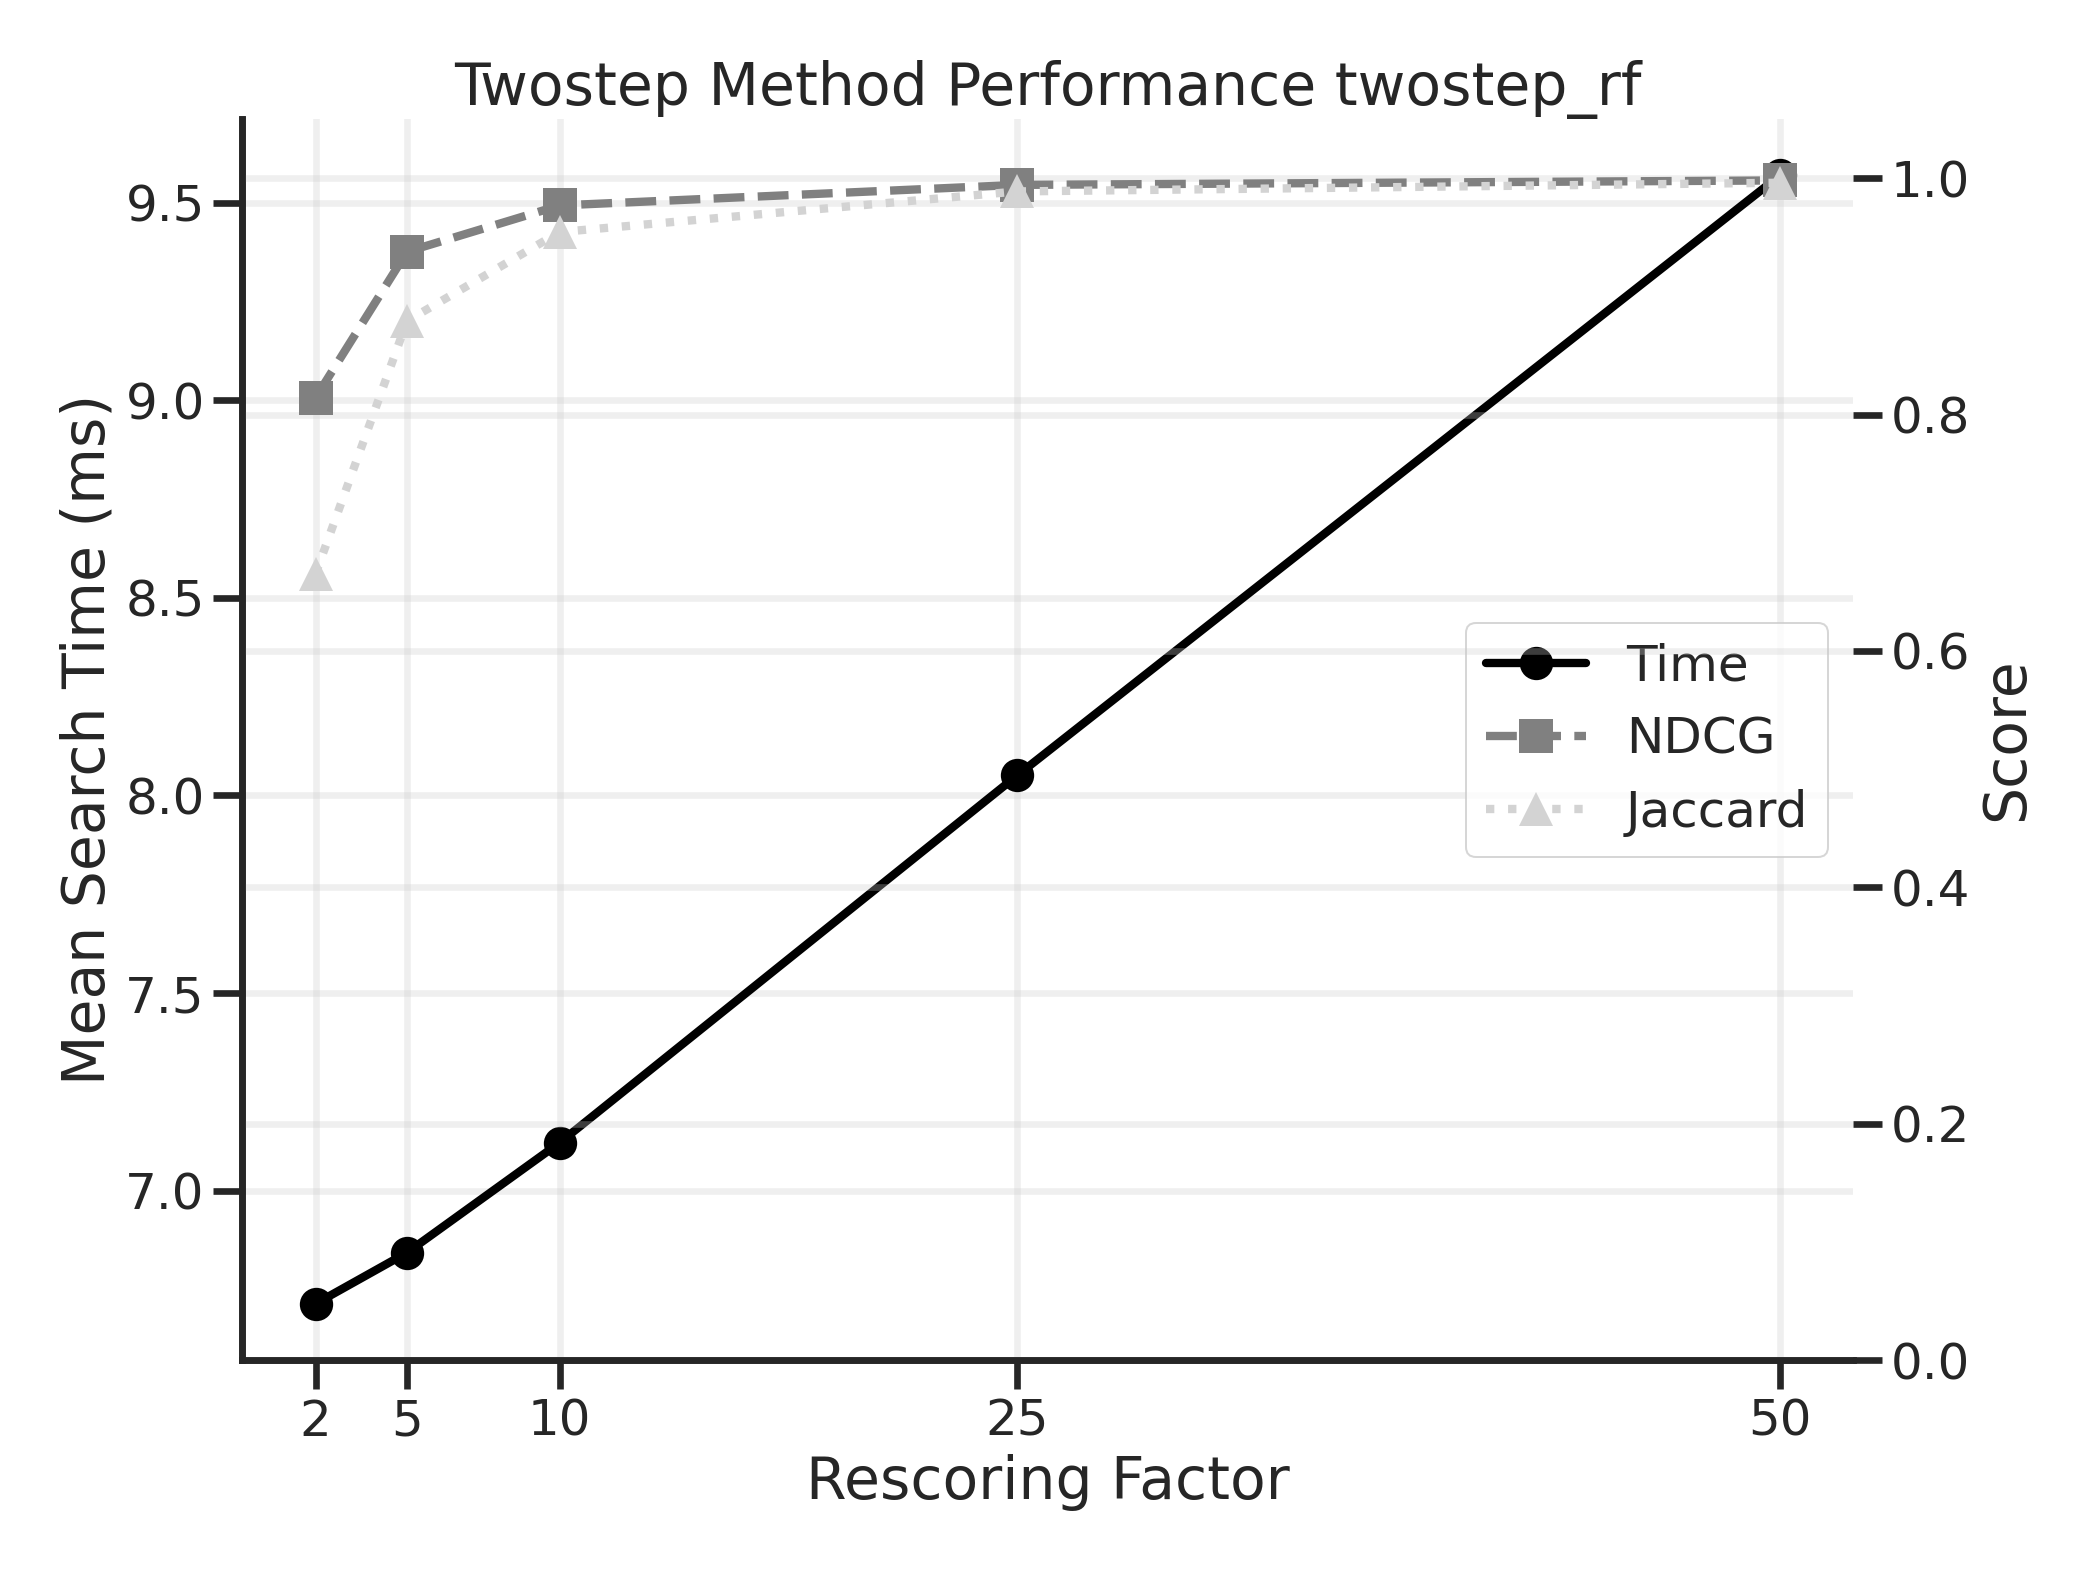
\includegraphics[width=0.49\widefigwidth]{bilder/plots/twostep_comparison_combined_benchmark_dim1024_k100_q.png}
            \vspace*{-1cm}
            \caption{\scriptsize{Time, NDCG, Jaccard vs Rescoring Factor Binary+Float}}
            \label{time_ndcg_jaccard_vs_rescoring_factor_bf}
        \end{minipage}
        %\hfill
        \begin{minipage}[t]{0.49\widefigwidth}
            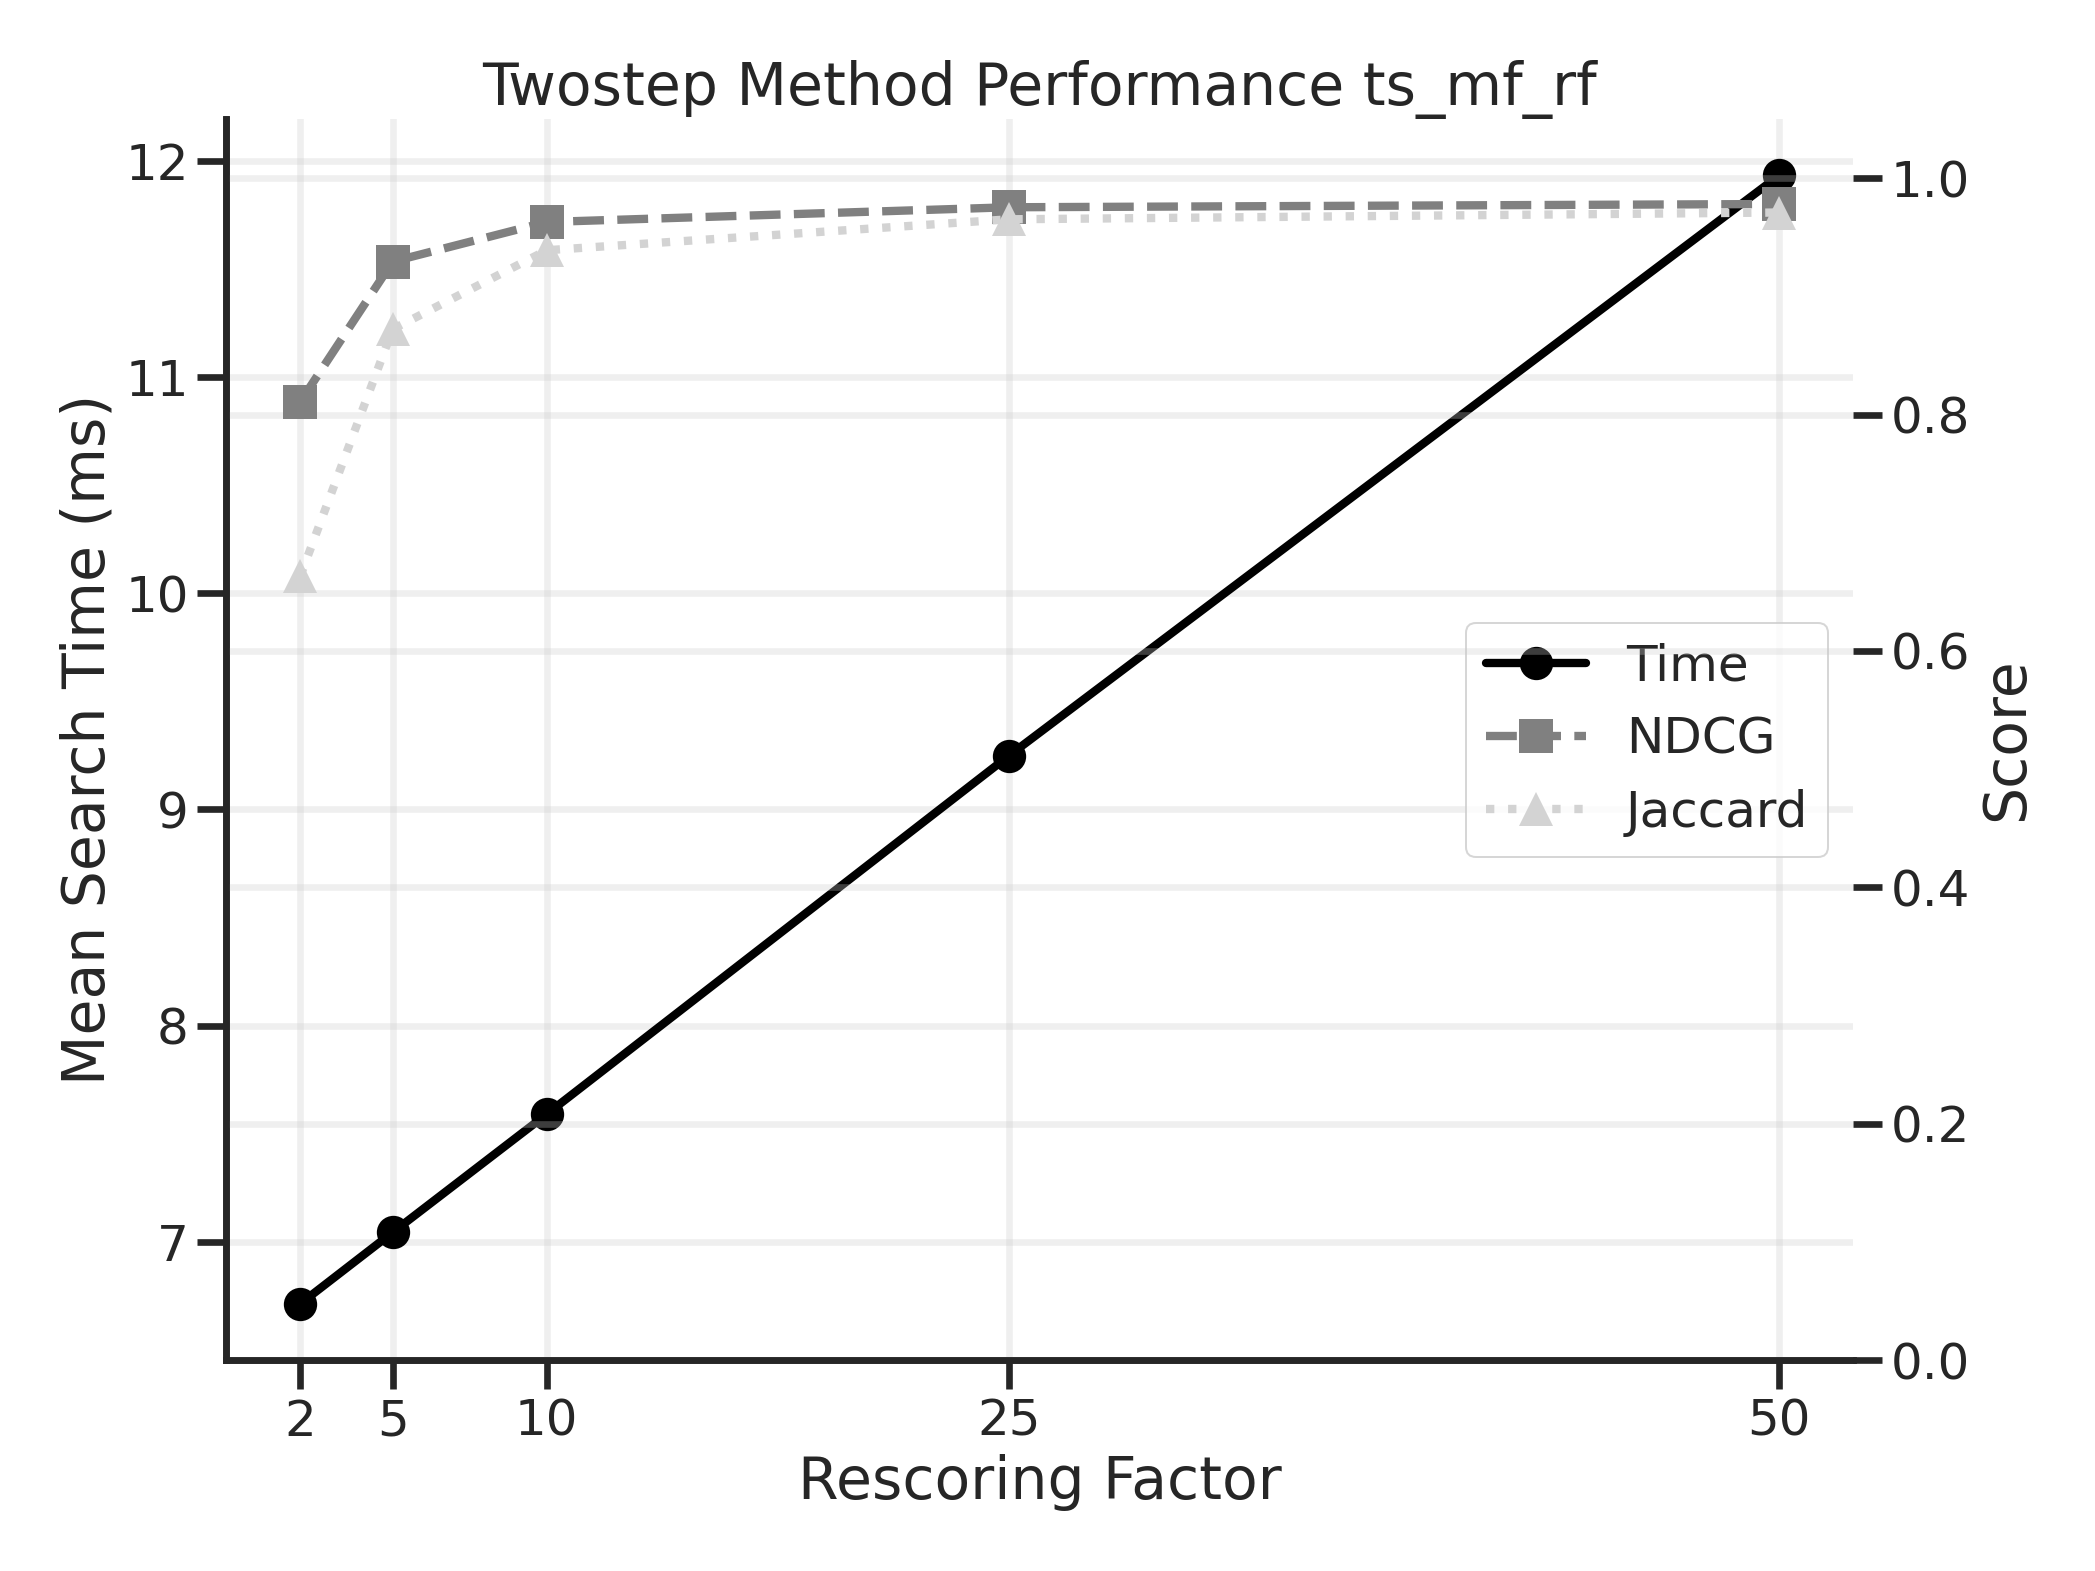
\includegraphics[width=0.49\widefigwidth]{bilder/plots/twostep_comparison_combined_benchmark_dim1024_k100_q_mf.png}
            \vspace*{-1cm}
            \caption{\scriptsize{Time, NDCG, Jaccard vs Rescoring Factor Binary+Mapped Float}}
            \label{time_ndcg_jaccard_vs_rescoring_factor_bmf}
        \end{minipage}
    }
\end{figure}

\subsection{Comparing Benchmark Results from Different Models}
\begin{figure}[h]
    \makebox[\textwidth][c]{%
        \begin{minipage}{0.49\widefigwidth}
            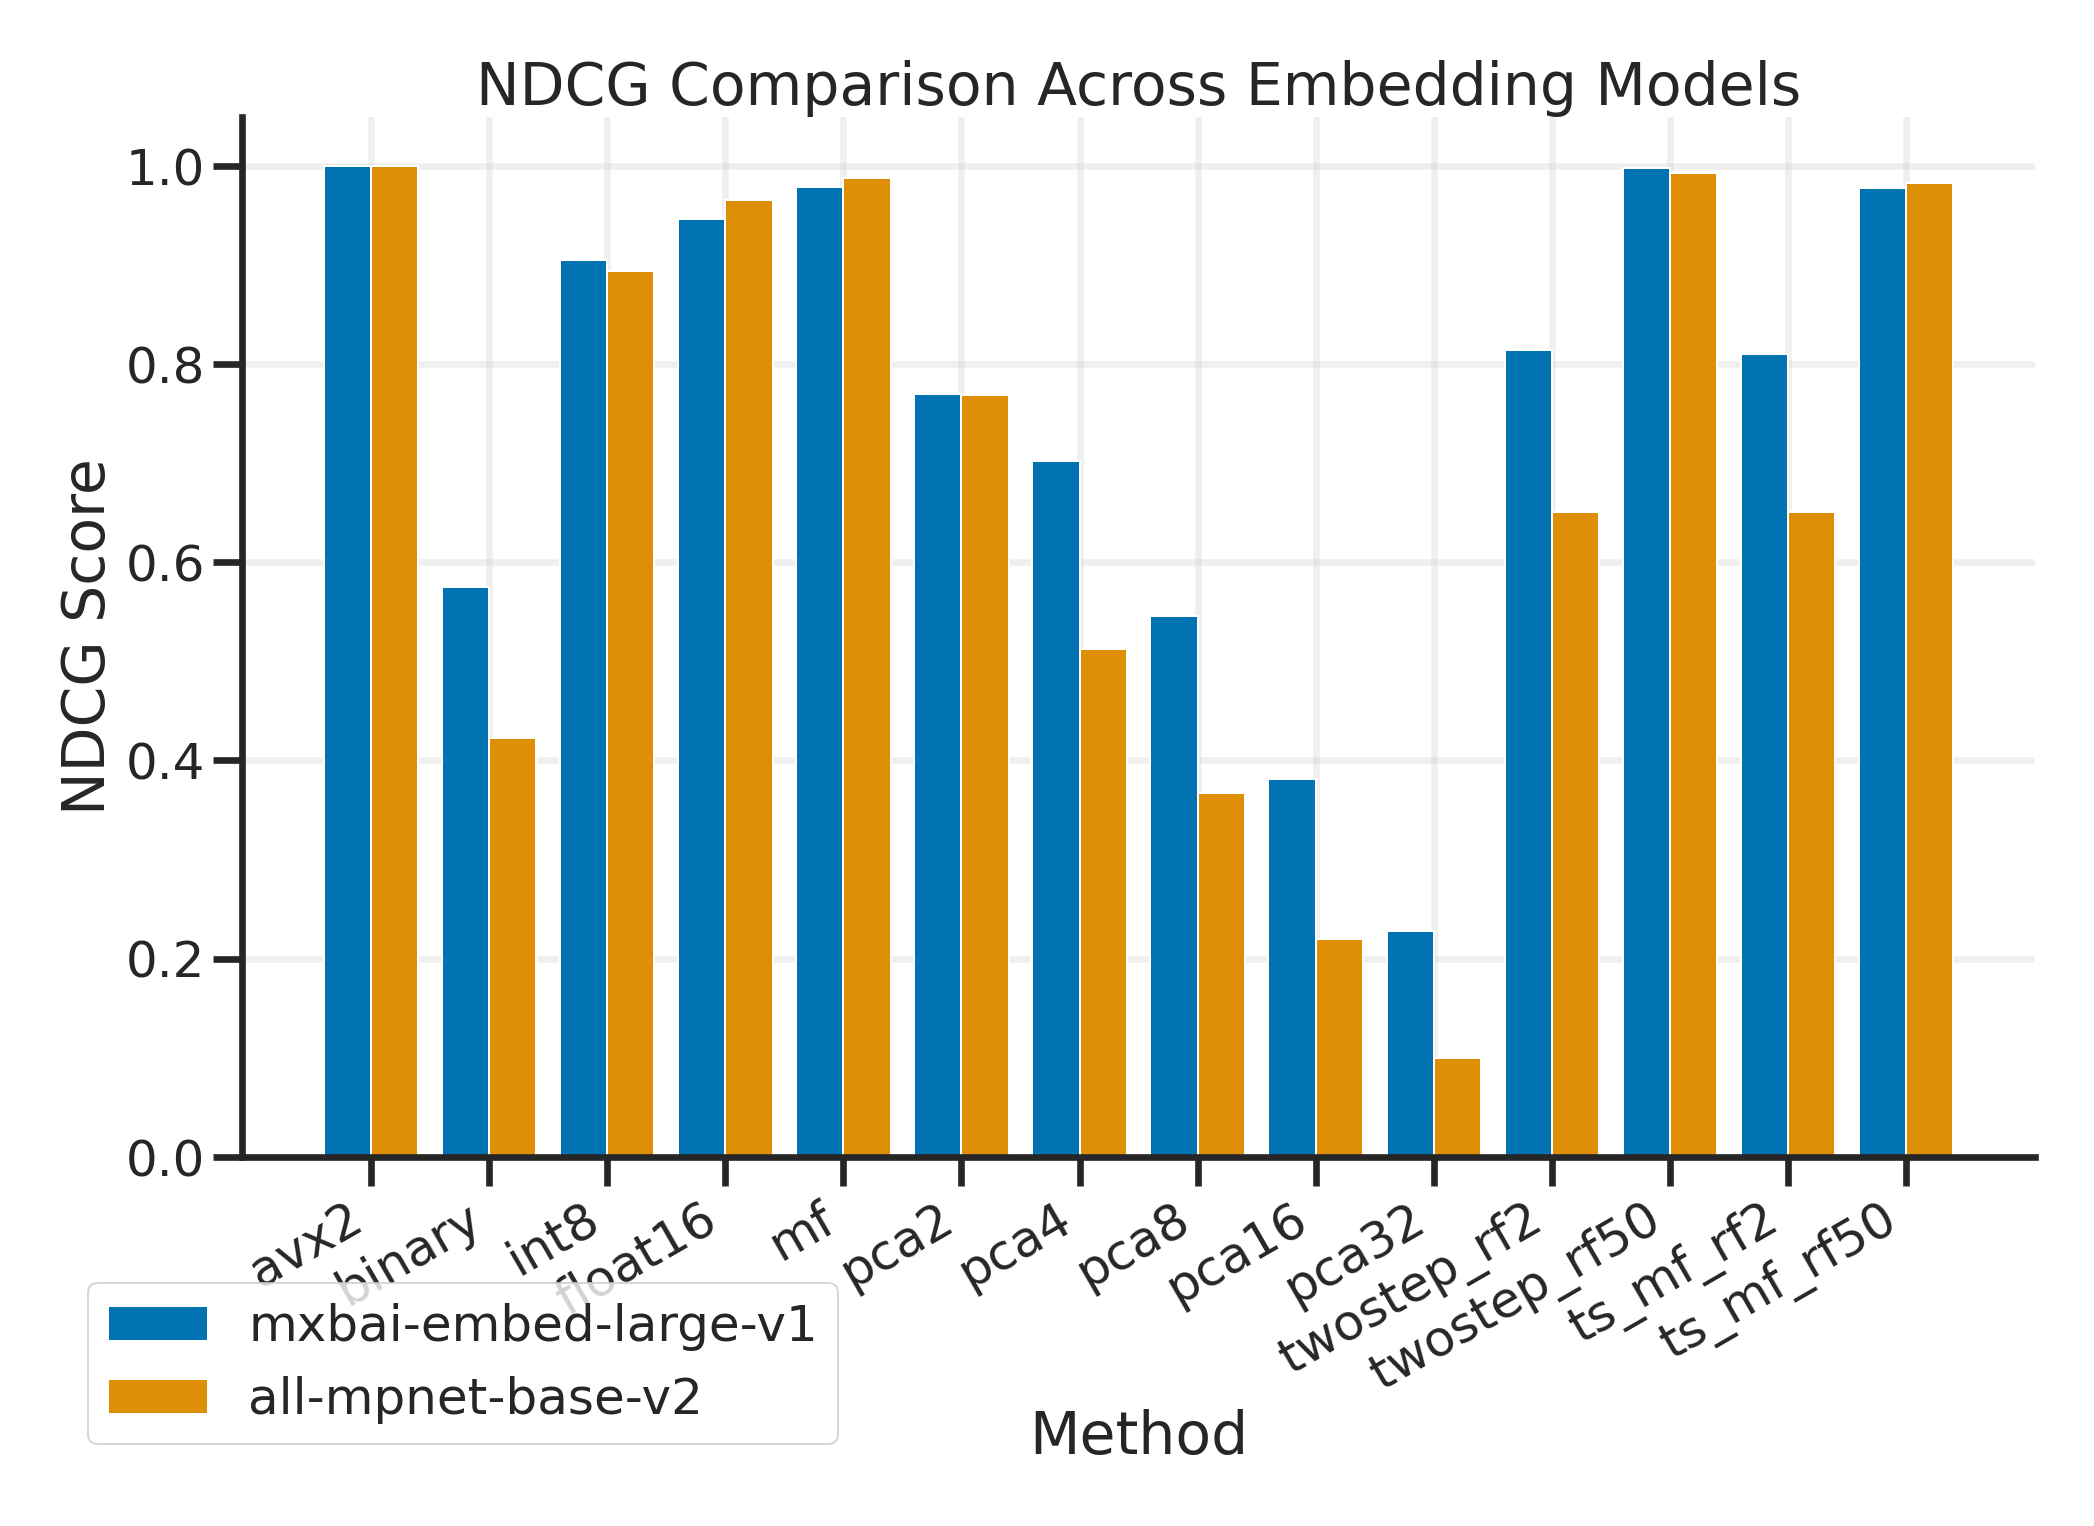
\includegraphics[width=0.49\widefigwidth]{bilder/plots/benchmark_comparison_dim1024_k100_q_dim768_k100_q.png}
            \vspace*{-1cm}
            \caption{\scriptsize{NDCG score comparison between different models}}
            \label{ndcg_comp_diff_models}
        \end{minipage}
        %\hfill
        \begin{minipage}{0.49\widefigwidth}
            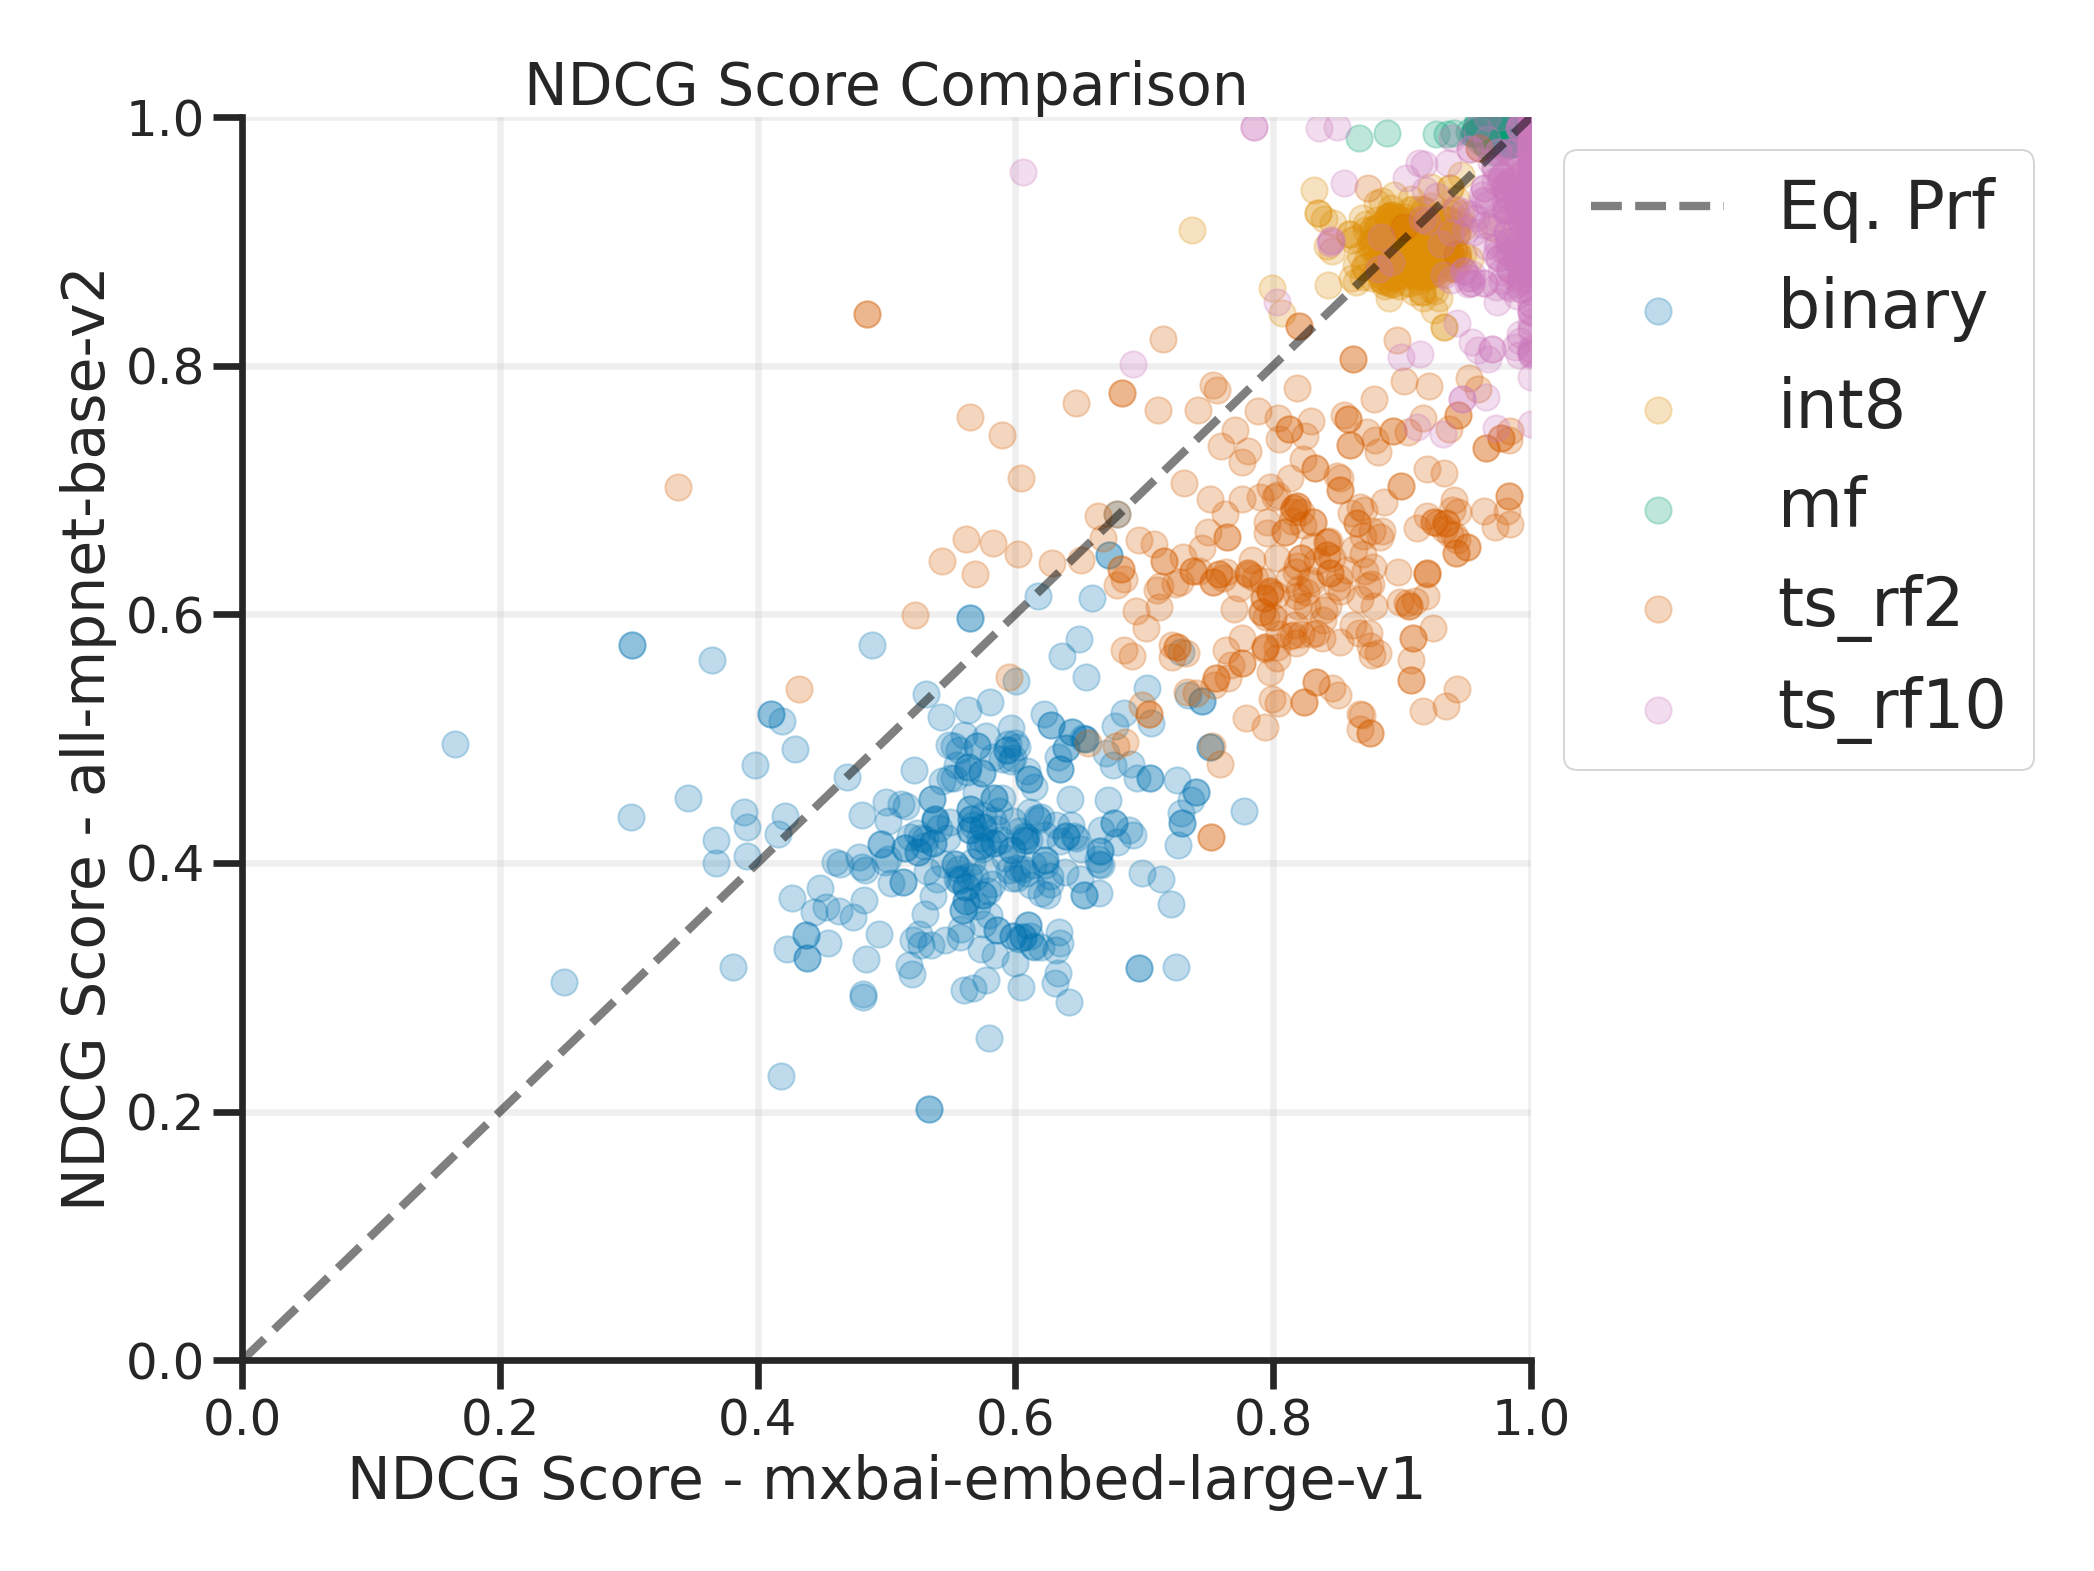
\includegraphics[width=0.49\widefigwidth]{bilder/plots/ndcg_scatter_benchmark_dim1024_k100_q_vs_benchmark_dim768_k100_q.png}
            \vspace*{-1cm}
            \caption{\scriptsize{NDCG score comparison between different models as scatter plot}}
            \label{ndcg_comp_diff_models_scatter}
        \end{minipage}
    }
\end{figure}
As mentioned earlier the model used is an angle optimized model, which should enable the binary searcher to get better results.~\cite{emb2024mxbai,li2024angleoptimizedtextembeddings}
To verify the previous results, the scores of the searchers when using the \texttt{\seqsplit{mixedbread-ai/mxbai-embed-large-v1}} model will be compared against the scores when using the \texttt{\seqsplit{sentence-transformers/all-mpnet-base-v2}} text embedding model. The same queries will be used.

Looking at the bar plot \autoref{ndcg_comp_diff_models} we see that the binary searcher indeed performs better with the angle optimized model. So does the two-step search as it's using the binary searcher in the first step. The PCA reduced searcher also perform better. This indicates, that the PCA algorithm is better at removing redundancies and grouping correlating dimensions for the embedding vectors created by the optimized model. There is no significant difference for the other searchers.

\subsection{Memory Usage Analysis}
\begin{figure}[h]
    \makebox[\textwidth][c]{%
        \begin{minipage}{0.49\widefigwidth}
            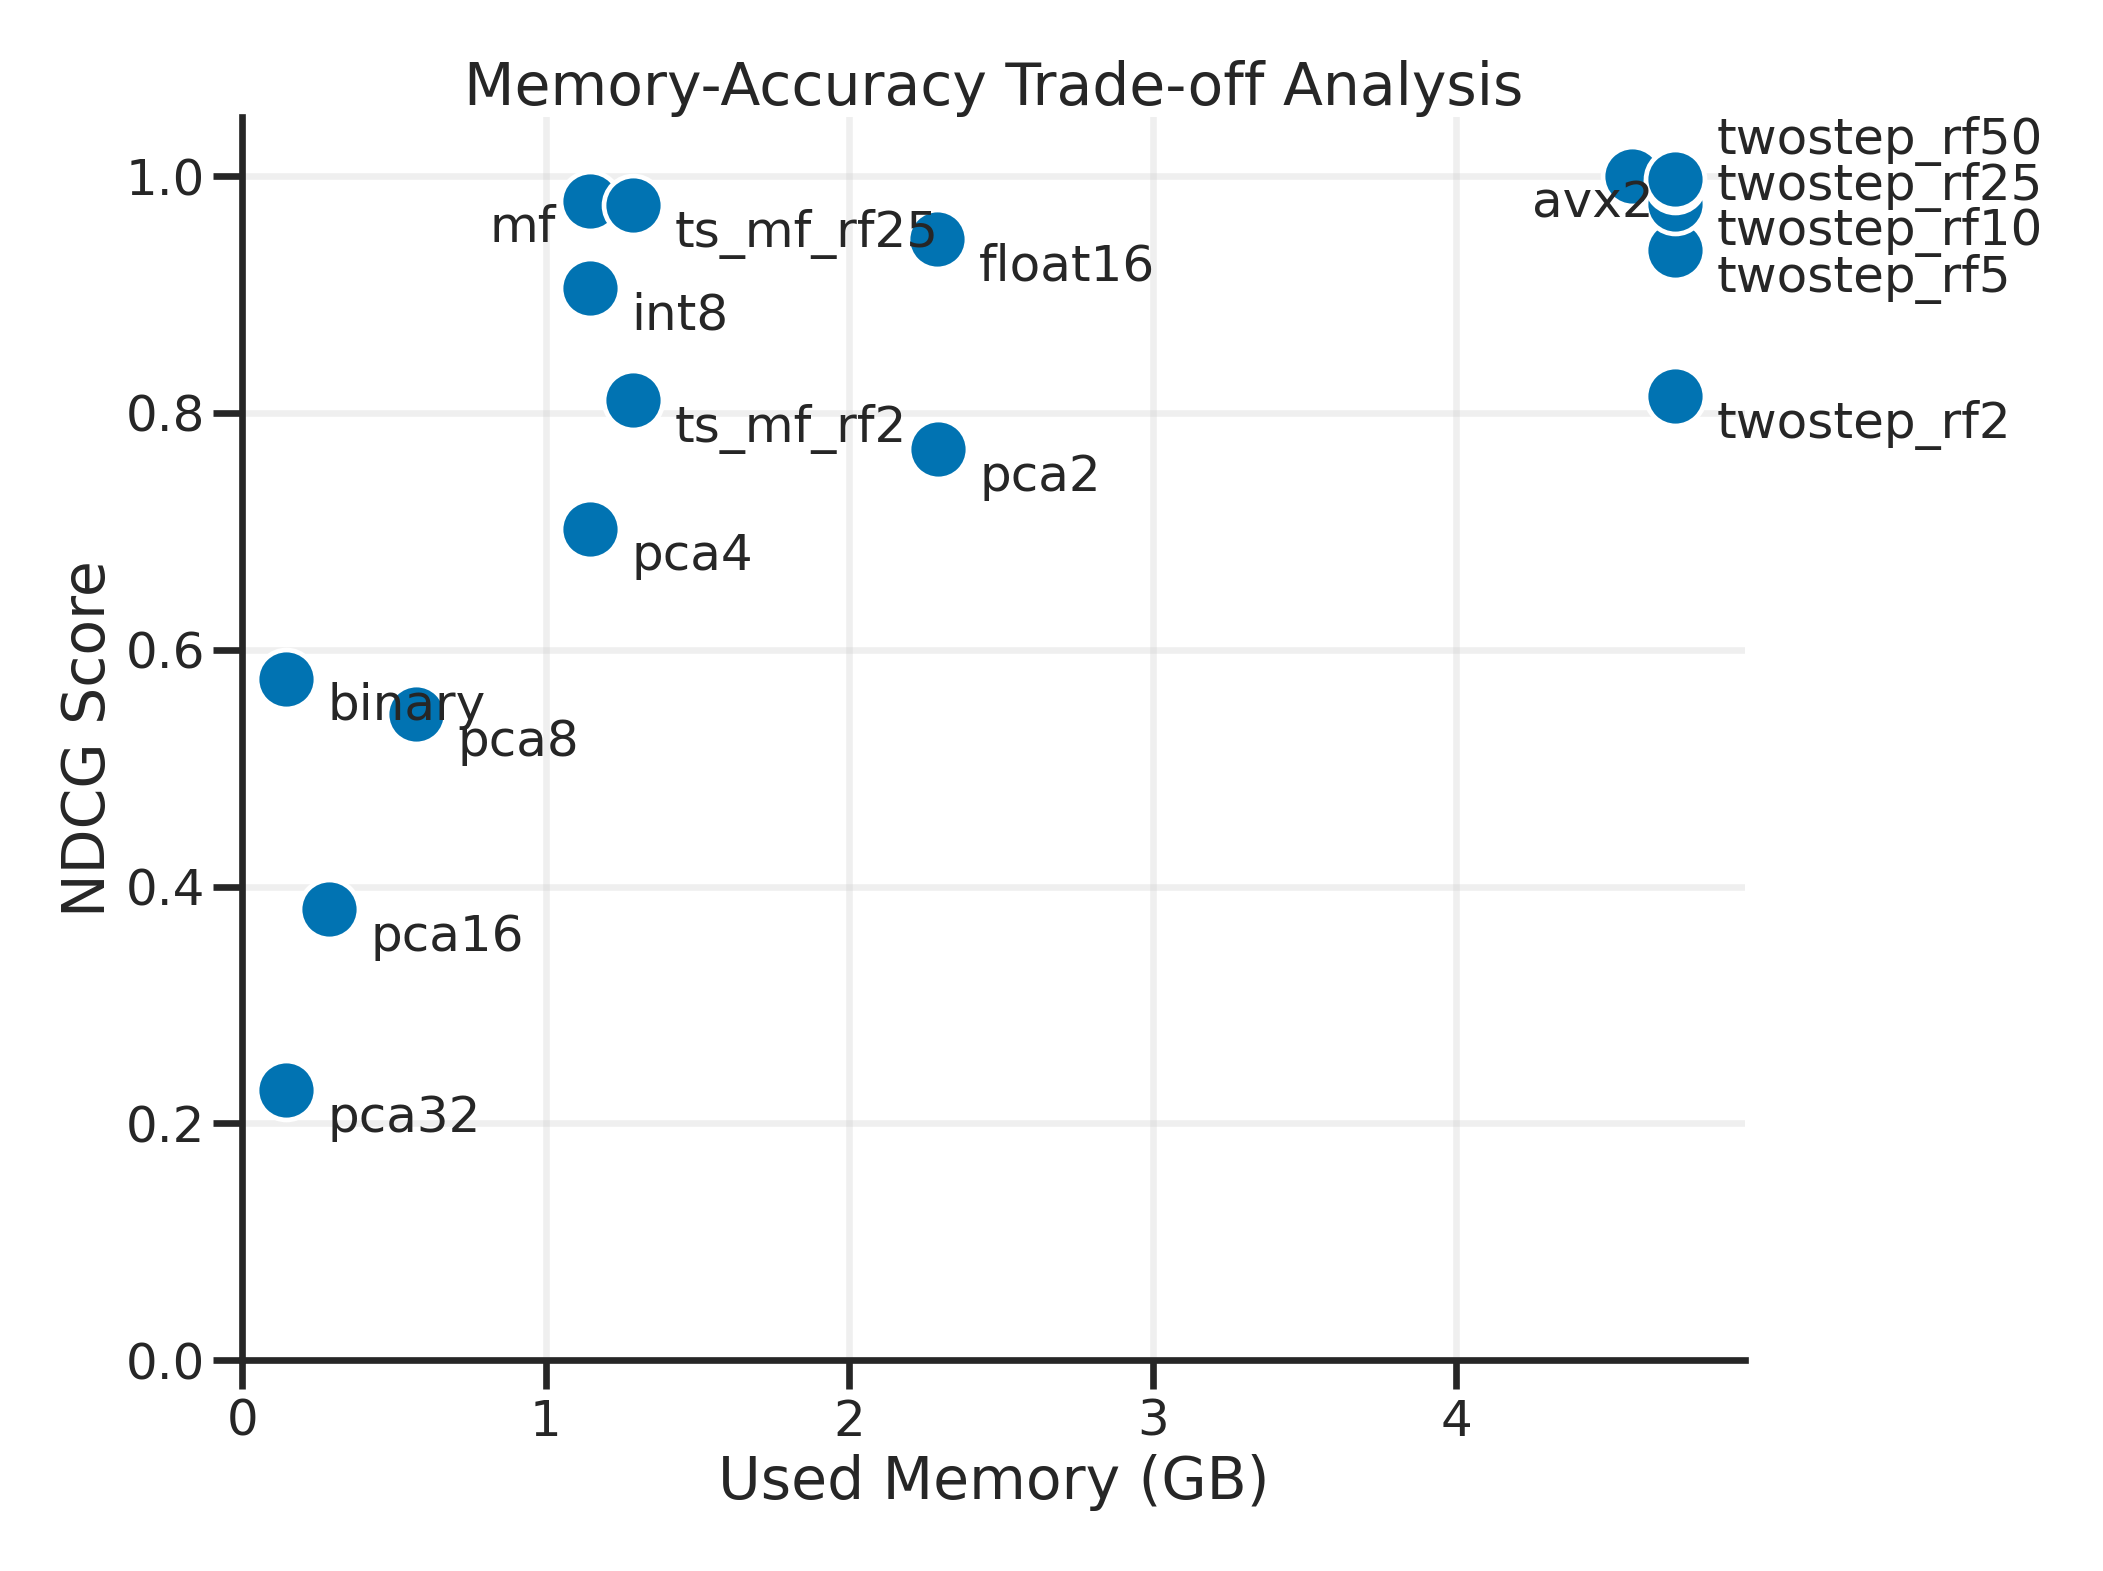
\includegraphics[width=0.49\widefigwidth]{bilder/plots/memory_vs_accuracy_dim1024_k100_q.png}
            \vspace*{-1cm}
            \caption{\scriptsize{NDCG Score vs Memory Usage}}
            \label{memory_vs_accuracy}
        \end{minipage}
        %\hfill
        \begin{minipage}{0.49\widefigwidth}
            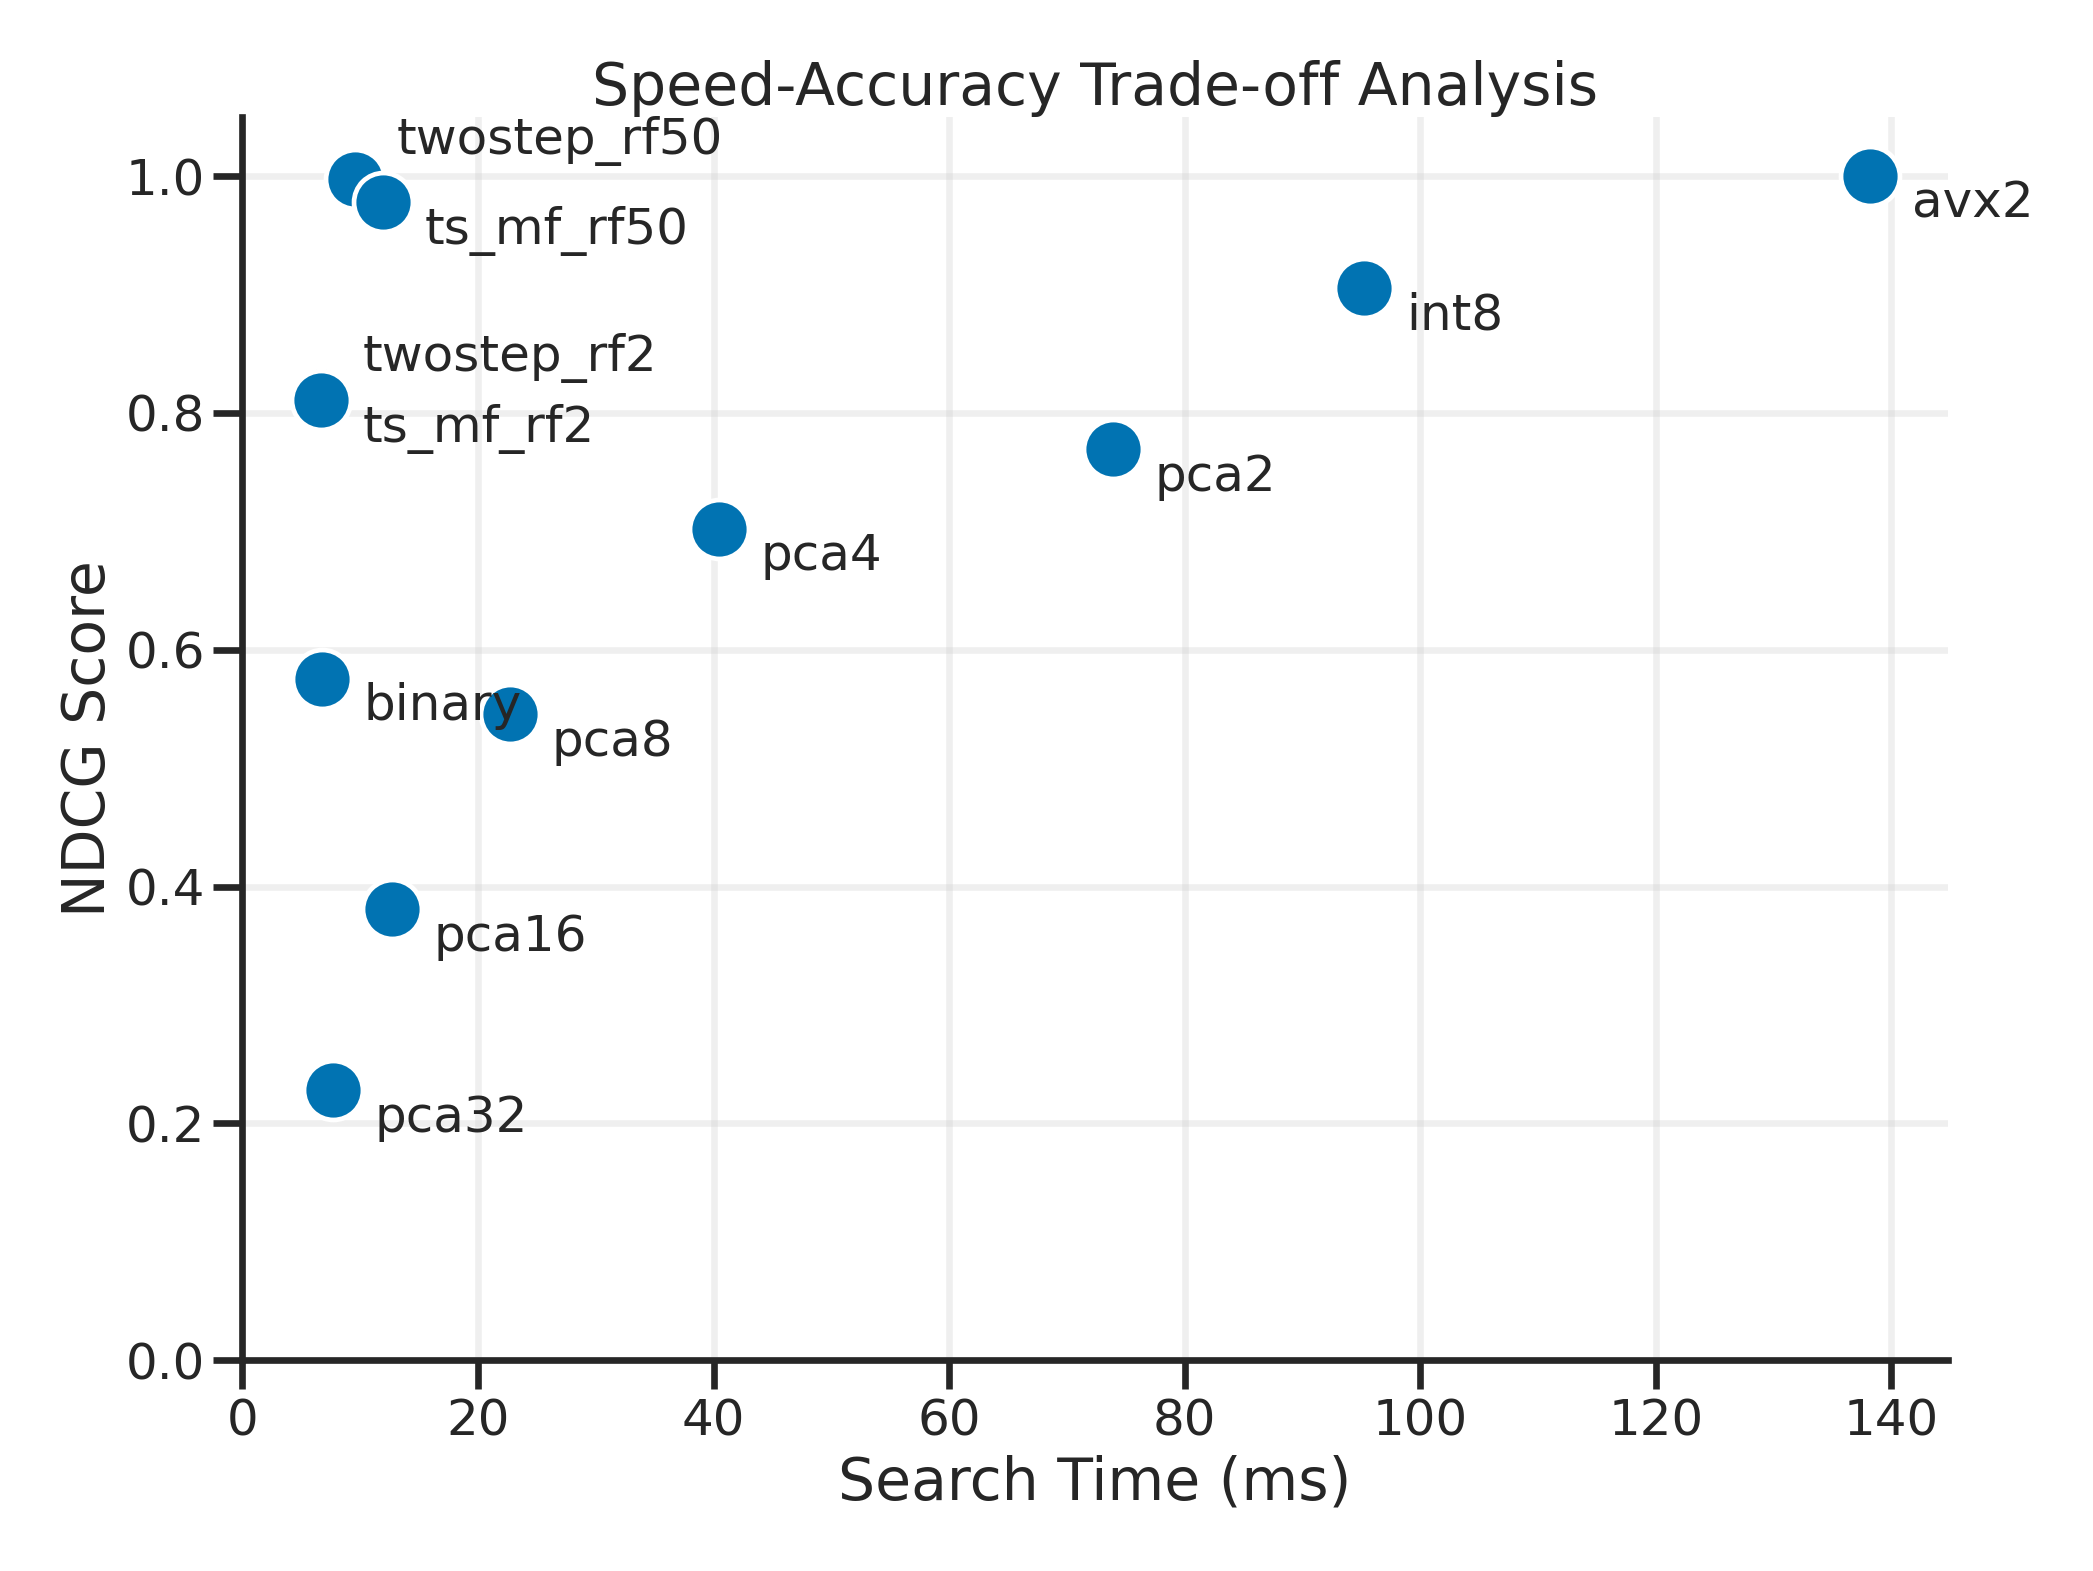
\includegraphics[width=0.49\widefigwidth]{bilder/plots/speed_vs_accuracy_dim1024_k100_q.png}
            \vspace*{-1cm}
            \caption{\scriptsize{NDCG Score vs Retrieval Time}}
            \label{memory_vs_speed}
        \end{minipage}
    }
\end{figure}
The binary+float searcher method uses the most memory, as it has to keep the binary and float32 embeddings in memory which totals to 33/32 times more memory usage compared to the baseline. Exactly the same memory usage as the baseline has the avx2 search, as it only optimizes the computation. And obviously the float16 variant uses half the memory of baseline.

The mapped float uses 1/4 of the baseline memory which makes it the best performing model in that memory range when factoring in its very high accuracy scores. This method is also one of the few not limited by memory bandwidth but by the L1 cache latency. Which makes it able to profit from multithreading on multicore CPUs as each core has its own L1 cache.

The binary+mapped float variant uses slightly more memory as it also has to load the binary embeddings, which, in return, makes it very fast. On its own the binary searcher uses the least memory except the PCA32 variant which has bad accuracy. The other PCA variants are also outperformed in search time and accuracy by other methods in the same memory range.

\subsection{Search Query Performance}
\begin{table}[h]
    \centering
    \begin{tabular}{l|ccccc|r}
        \toprule
        Query                                                           & \multicolumn{5}{c}{NDCG score} & type                                    \\
        \hline
                                                                        & binary                         & int8  & mf    & pca4  & ts\_rf10 &      \\
        \hline
        :)                                                              & 0.250                          & 0.799 & 0.867 & 0.202 & 0.691    & bad  \\
        paper                                                           & 0.302                          & 0.835 & 0.958 & 0.366 & 0.785    & bad  \\
        maps of places that don't exist yet                             & 0.392                          & 0.846 & 0.941 & 0.546 & 0.844    & bad  \\
        history of the number zero                                      & 0.464                          & 0.907 & 0.971 & 0.564 & 0.918    & bad  \\
        cars                                                            & 0.489                          & 0.881 & 0.957 & 0.623 & 0.966    & var  \\
        \footnotesize evolution of human color vision and its gene...   & 0.584                          & 0.921 & 0.984 & 0.691 & 1.000    & var  \\
        sun                                                             & 0.617                          & 0.892 & 0.982 & 0.575 & 1.000    & var  \\
        \footnotesize archaeological evidence of prehistoric human...   & 0.570                          & 0.878 & 0.990 & 0.720 & 1.000    & rand \\
        \scriptsize PLEASE HELP ME FIND INF[...] ABOUT DOLPHINS!!!      & 0.598                          & 0.914 & 0.978 & 0.791 & 0.976    & rand \\
        Roman legion size                                               & 0.604                          & 0.937 & 0.986 & 0.786 & 1.000    & good \\
        \footnotesize development of early mechanical calculators in... & 0.575                          & 0.938 & 0.990 & 0.770 & 1.000    & good \\
        pizza pizza pizza pizza pizza pizza pizza                       & 0.778                          & 0.971 & 0.995 & 0.839 & 1.000    & good \\
        \bottomrule
    \end{tabular}
    \caption{Accuracy for different search queries}
    \label{queryanalysis}
\end{table}

In the \autoref{queryanalysis} are some queries listed that were also used in the benchmarks. The table lists the corresponding scores for some search implementations. 4 categories of queries were selected: Good and bad performing queries, queries with high score variance and randomly selected queries. The worst performing query is just a ":)" it's an unconventional query that has no point. Even a human would have problems interpreting a distinct semantic meaning into it. But still, the int8, mapped float and two-step method perform quiet well. The binary and PCA4 score is with around 0.2 really low. But this explains the big outliers in the box plots \ref{boxjaccardsearchersone} \ref{boxndcgsearchersone} \ref{boxjaccardsearcherstwo} \ref{boxndcgsearcherstwo}. Which makes the outliers less bad, because you can't expect good results from a query like this. "paper", a really generic query that also has quiet low scores, especially for the binary and PCA4 searcher. The other implementations perform good enough with this query. An example for more specific queries would be "Roman legion size". Here its very apparent what the user would want as an answer. All searchers have good score with this query.

In conclusion, more specific queries, which also implies more semantic meaning, seem to perform better. It also explains the outliers of the lower accuracy models and gives more confidence in rating them as usable.



\section{Summary}
Most results are roughly in line with the expectations. The accuracy of the mapped float searcher is very surprising. The fact it performs better than float16 with only 8 bits was unexpected. But the reason for this could be the accuracy loss during float addition. During the calculation of the dot product the products of the vector dimensions are added to the dot product where each addition can generate accuracy loss. And for the float16 this running sum is also in float16 format, while the mapped float uses float32 for this, as its using float32 values during multiplication.

The slow speed of the int8 search can be explained by the instruction intensive splitting, moving and extending of vectors/values, which is needed to prevent overflow. Maybe quantization with a limit of 4 used bits would be better, as one could then simply multiply the int8 values without risking overflow.

PCA performed much worse than expected as even PCA2s accuracy is outperformed by simple int8 quantization.

Also, the binary and two-step methods are overall the most useful as they are very fast. For the two-step methods comes the addition of being very accurate. And two-step with the mapped float even hast a fairly low memory usage which makes it overall the best performers when considering all 3 main metrics of memory usage, accuracy and speed.